\documentclass[12pt]{article}
\usepackage{xcolor,graphicx}
\usepackage{hyperref}
\usepackage{wasysym}
\textwidth 17cm
\oddsidemargin -0.54cm  %2cm Rand links
\topmargin 0.46cm %3cm Rand oben
\headheight 0cm % no header
\headsep 0cm
\textheight 22cm
\parskip 3pt
\parindent 0pt
\sloppy

\definecolor{cadmiumgreen}{rgb}{0.0, 0.42, 0.24}
\definecolor{burntorange}{rgb}{0.8, 0.33, 0.0}

\newcommand{\redast}{{\color{red}\ast}}

\newcommand\code[1]{{\tt #1}}

\newcommand{\ofld}[1]{\colorbox{black!15}{{\bf #1}}}
\newcommand{\ofldx}[1]{\colorbox{black!15}{(#1)}}

\newcommand\guico[1]{{\color{blue}\code{#1}}}
\newcommand\guifco[1]{{\color{violet}\code{#1}}}
\newcommand{\unico}[1]{{\color{burntorange}\code{#1}}}

\newcommand{\evcod}[2]{\ofld{#1} $\rightarrow$ \guico{#2}}
\newcommand{\evcodx}[2]{\ofldx{#1} $\rightarrow$ \guico{#2}}
\newcommand{\evcodf}[2]{\ofld{#1} $\rightarrow$ \guifco{#2}}
\newcommand{\evcodxf}[2]{\ofldx{#1}~$\rightarrow$ \guifco{#2}}
\newcommand{\prcod}[2]{\opauni{#1}$>$\unico{#2}}
\newcommand{\vrcod}[2]{\opauni{#1}:\unico{#2}}
\newcommand{\grcod}[2]{\opagui{#1}$>$\guico{#2}}
\newcommand{\gfcod}[2]{\opaguif{#1}$>$\guifco{#2}}

\newcommand{\opagui}[1]{\colorbox{blue!20}{{\color{black}\code{#1}}}}
%\newcommand{\opagui}[1]{\fbox{\code{#1}}}
%\newcommand{\oguih}[1]{{\Huge ~\\ \label{#1}{\opagui{#1}}}\\}
\newcommand{\oguih}[2]{\subsection{\label{#2}#1}{\Huge\opagui{#2}}\\}
\newcommand{\ogui}[1]{\hyperref[#1]{\opagui{#1}}}

\newcommand{\opaguif}[1]{\colorbox{violet!30}{{\color{black}\code{#1}}}}
%\newcommand{\oguifh}[1]{\subsection{\Huge\label{#1}{\opaguif{#1}}}}
\newcommand{\oguifh}[2]{\subsection{\label{#2}#1}{\Huge\opaguif{#2}}\\}
\newcommand{\oguif}[1]{\hyperref[#1]{\opaguif{#1}}}


\newcommand{\opauni}[1]{\colorbox{orange!30}{{\color{black}\code{#1}}}}
%\newcommand{\opauni}[1]{\underline{\code{#1}}}
%\newcommand{\ounih}[1]{\subsection{\Huge\label{#1}{\opauni{#1}}}}
\newcommand{\ounih}[2]{\subsection{\label{#2}#1}{\Huge\opauni{#2}}\\}
\newcommand{\ouni}[1]{\hyperref[#1]{\opauni{#1}}}

\newcommand{\tabouni}[1]{\ref{#1} & \ouni{#1}}
\newcommand{\tabogui}[1]{\ref{#1} & \ogui{#1}}
\newcommand{\taboguif}[1]{\ref{#1} & \oguif{#1}}


%\newcommand{\uses}[1]{\subsubsection{Uses} #1}
%\newcommand{\uses}[1]{\rule[3pt]{\textwidth}{0.2pt} \\ {\bf Uses: } #1}
\newcommand{\uses}[1]{\flushleft {\bf Uses:} #1}

%\newcommand{\desc}[1]{\subsubsection*{Description} #1}
\newcommand{\desc}[1]{#1}
\newcommand{\act}[1]{\subsubsection*{Actions} #1}
\newcommand{\pvar}[1]{\subsubsection*{Public constants, types and variables} #1}
\newcommand{\ppro}[1]{\subsubsection*{Public procedures} #1}

\newcommand{\todo}[1]{{\color{red} #1}}
\newcommand{\feature}[1]{{\color{cadmiumgreen} #1}}

\newcommand{\biburl}[1]{{\small{\tt #1}}}


\newcommand\opamodule[3]{{\bf \tt #1} #2\\  \rule[3pt]{\textwidth}{0.2pt} \\ {\scriptsize uses \tt  #3}\\[1ex]}
\newcommand\opamoduleN[2]{{\bf \tt #1} #2\\  \rule[3pt]{\textwidth}{0.2pt} \\}

\newcommand{\see}{\mbox{$\rightarrow$}}


\begin{document}\noindent
\fboxsep1pt

\parbox[t]{0.7\hsize}{
  {\Huge\bf OPA documentation} version {\bf 4.2.0}\\
  Andreas Streun, \today
} \hfill  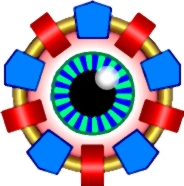
\includegraphics{opalogo_small.jpg}
\rule{\hsize}{1pt}

\section{How to use this document}
This document is intended to support program developers, who want to maintain the existing OPA code, or to rewrite it in another environment, or to extract useful parts for integration into other codes.

When reading this document, the source code may be examined in parallel, preferably in the Lazarus IDE. In order to see how the code works, OPA may be executed or the tutorial \cite{tutorial} may be consulted. Further information on using OPA is found in the user guide \cite{userguide} and the underlying physics is outlined in \cite{inside}.

In this document following styles are used:\\
Pieces of code are shown in \code{typewriter style}.
\opagui{GUI} is a graphical user interface, usually based on class \code{TForm}. \opaguif{Frame} if a user-defined GUI-component, usually based on class \code{TFrame}.  \opauni{Unit} is a standard Pascal unit.  

A GUI or a frame has a list of \guico{actions} corresponding to the event handlers of its components, for example a button to be pressed. The pure Pascal units are passive, they contain a set of public \unico{procedures} which are called from the GUIs. Frames too may contain public \guifco{procedures}. Thus in this documentation, action lists are given for the GUIs and frames, and lists of public procedures for the frames and units. All modules may offer public variables, here coloured \guico{x}, \guifco{y}, \unico{z} for GUIs, frames, units.

GUI components accept user input and/or launch events. Some have captions, like \ofld{Buttons}, others not, like for example a \ofldx{plot area} responding to mouse clicks. The general scheme is \evcod{component}{event handler}. Event handlers may call private procedures of the GUI or public procedures from units as listed in the \guico{uses} section. For the units \prcod{unit}{procedure} refers to a procedure in a unit and \vrcod{unit}{variable} to a public variable..

\todo{Red text gives informations about bugs and other problems and/or suggestions for future improvements.} \feature{Green text mentions particular features which distinguish OPA from other beam dynamics codes and should be preserved.}

Questions may be adressed to the author at \url{mailto:psi@andreas-streun.de}.

%\opamust indicates that this part of the code is essential and should be included
\newpage


\section{OPA status}

Following semantic versioning \cite{semver} version 4.063 of OPA was renamed 4.1.0. However, since up to now only the author worked on the code, the distinctions MAJOR, MINOR, PATCH rather refer to the changes as visible to the users than to the API. 


Current version is OPA 4.2.1. It includes 44 Pascal units \code{.pas}, 29 of them are \opagui{GUIs} which are accompanied by a Lazarus form \code{.lfm} (created by the Lazarus IDE), and 15 of them are Pascal \opauni{units}. Four of the GUIs are \opaguif{frames}, i.e. self-defined components embedded in other GUIs. Four units are located in a parallel folder, here called \code{../com/} since they are not OPA specific but used with other programs too.
Table~\ref{tabover} lists the units. The column "Size" lists the lines of code as a rough estimate for the complexity of the unit. Furthermore, OPA includes the main program file \ouni{opa.lpr} and a couple of image files \code{.ico, .bmp} to draw symbols on buttons. 

A GUI defines a class, given in table~\ref{tabover} in the column "class". The actual GUI is the one and only instance of this class, i.e. a public variable, usually with the name as the class but without the leading "T". A frame also defines a class but no instance, instead the parent GUI will define one or more instances of this class as variables. A standard Pascal unit may also define a class to be instantiated, or it is a library, i.e. a collection of variables and public procedures.

In general GUIs should handle the user interactions only while the Pascal units do all the calculations. This separation was largely realized in OPA, however not strictly. Some minor calculations are done in the GUI in some places.

In version 4.2.0 all files were renamed following this convention for the file name: 
\code{opa*} is a first level GUIs, i.e. one of the main design programs launched from the main menu. \code{*lib} is a plain Pascal units which contains a library of physics procedures. 
\code{o*} is a second level GUI, which is launched by a first level GUIs, for example a start menu. \code{*frame} is a frame. Files in the \code{../com} folder were not renamed. \\

Table~\ref{tabover} also serves as a {\bf table of contents} with the first column listing the section numbers:
Section \ref{secglob} will explain the "backbone" of OPA, which are the global datatypes and variables, the main menu and units for mathematics and graphics which are used by many GUIs. 
Section \ref{secedit} contains lattice file handling and the two editors, text-based and "LEGO" block like.

Beam physics starts with section \ref{seclino} on the interactive linear optics design panel and related GUIs and units and continues with section~\ref{secmomo} on off-momentum optics and bucket viewer. The non-linear optimization module is explained in section~\ref{secnonl}, and section~\ref{secorin} covers injection and orbit correction.

The three tracking modules with their library are explained in section \ref{sectrac}. Section~\ref{secspee} contains an editor for longitudinal gradient bends. Finally, machine layout and magnet currents are in section~\ref{secelse}.






\begin{table}
\caption{OPA units overview}
\label{tabover}
{\small
\begin{tabular}{llllr}
Sec & Name & class & Purpose & Size \\ \hline
\tabouni{globlib} & & global variables and procedures & 2986 \\
\tabogui{opamenu} & \guico{TMenuForm} & the main menu & 901 \\
\tabouni{mathlib} & & mathematical library & 2075 \\
\tabouni{../com/vgraph} & \unico{Vplot} & real number graphics library & 1276 \\
\taboguif{../com/asfigure} & \guifco{TFigure} & general plot procedure & 314 \\
\tabouni{../com/conrect} & & contour plot calculation & 332 \\
\tabouni{../com/asaux} & & little helpers & 349 \\
\hline
\tabouni{latfilelib} & & file reading and writing & 1839 \\
\tabogui{opatexteditor} & \guico{TFormTxtEdt} & text editor for lattice file & 190 \\
\tabogui{opaeditor} & \guico{TFormEdit} & interactive lattice editor  & 346 \\
\tabogui{oelecreate} & \guico{TEditElemCreate} & creation of an element & 144 \\
\tabogui{oeleedit} & \guico{TEditElemSet} & edit element parameters & 861 \\
\tabogui{osegedit} & \guico{TEditSegSet} & edit segment parameters & 444 \\
\hline
\tabogui{opalinop} & \guico{Toptic} & linear optics design & 1143 \\
\taboguif{knobframe} & \guifco{TKnob} & slider to set element property & 421 \\
\tabogui{ostartmenu} & \guico{Tstartsel} & setting for start parameters & 615 \\
\tabogui{obetenvmag} & \guico{TsetEnvel} & setting for optical functions plot & 372 \\
\tabogui{otunematrix} & \guico{TtuneMatrix} & adjustment of lattice tune & 251 \\
\tabogui{owriteomrk} & \guico{TWOMK} & write optics markers & 125 \\
\tabouni{linoplib} & & linear beam dynamics calculations & 2840 \\
\tabouni{elemlib} & & element propagation calculations & 2387 \\
\tabogui{omatching} & \guico{TMatch} & linear optics matching & 1457 \\
\tabogui{omatchscan} & \guico{TsetMatchScan}& parameter scan & 119 \\
\tabogui{opatunediag} & \guico{TTunePlot} & show the tune diagram & 634 \\
\hline
\tabogui{opamomentum} & \guico{Tmomentum} & momentum dependence and optimization & 949 \\
\tabouni{momentumlib} &  & momentum dependent calculations & 480 \\
\tabogui{opabucket} & \guico{TBucketView} & plot RF bucket & 640 \\
\hline
\tabogui{opachroma} & \guico{TChroma} & nonlinear optimization & 1413 \\
\taboguif{csexframe} & \guico{TCSex} & controller for nonlinear element & 454 \\
\taboguif{chamframe} & \guico{TCHam} & bar indicator for Hamiltonian mode & 416 \\
\tabouni{chromreslib} & & little helper to pass results handles & 79 \\
\tabouni{chromelelib} & & little helper to pass element handles & 93 \\
\tabogui{ochromsvector} & \guico{TSVectorPlot} & show Hamiltonian as complex vector & 145 \\
\tabouni{chromlib} & & nonlinear dynamics calculations & 1813 \\
\hline
\tabogui{opaorbit} & \guico{TOrbit} & orbit correction and injection & 2353 \\
\hline
\tabogui{opatrackps} & \guico{} & phase space tracking & 1422 \\
\tabogui{opatrackda} & \guico{} & dynamic aperture tracking & 1666 \\
\tabogui{opatracktt} & \guico{} & Touschek tracking & 1726 \\
\tabouni{tracklib} & & particle tracking calculations & 1502 \\
\hline
\tabogui{opalgbedit} & \guico{} & longitudinal gradient bend editor & 702 \\
\tabouni{lgbeditlib} & & longitudinal gradient bend calculations & 471 \\
\hline
\tabogui{opageometry} & \guico{} & geometric machine layout and matching & 2010 \\
\tabogui{opacurrents} & \guico{} & export magnet currents to machine control & 303 \\
\tabouni{testcode} & & test of new features & 472 
\end{tabular}
}
\end{table}

\pagebreak

\section{\label{secglob}Main programs and general use}

\ounih{Main program}{{opa.lpr}}

\desc{The main program file which allocates the units as described below and creates some of the forms. It is created more or less automatically by the Lazarus IDE.}


\ounih{Global data}{globlib}

\desc{
This unit defines global constants, types and variables and thus is OPA's "database". It is also initialized first when OPA starts and sets environment variables and default values. Public variables defined here are used by the other modules, since almost all of them use \ouni{globlib}. These "global" variables contain the basic lattice data, status flags, handles to access GUI components and temporary data to be exchanged between modules. This unit also provides many public procedures for various non-physics tasks. Only an overview can be given here, and the most important or complex things will be explained. Everything else should become clear from the code, hopefully.

\todo{The \ouni{globlib} unit grew large large and heterogenous over the years and should be split into several units for the different functions to be performed, or procedures should be moved to other units if applicable.}

Like other beam dynamics programs OPA works on a lattice file. It contains {\em elements}, mainly magnets of different type, and {\em segments}, which are line-ups of elements and segments. One of the segments is selected and expanded to become {\em the lattice} to work with. Element parameters, e.g. quadrupole strength in the lattice file can be numbers or arithmetic expressions using {\em variables}, which are part of the lattice file too.
}

\uses{\opauni{../com/mathlib}, \opauni{../com/asaux}}

\pvar{
Constants include general settings, array sizes, color definitions, name strings and values of flags later to be referenced by name.\\

Following type definitions may be considered as non-trivial:

\unico{ElementType} is a case-record for defining element parameters such as length, quad focusing strength, dipole bending angle etc. Several (but not all) parameters may be arithmetic expressions instead of numbers. For more details see the user guide \cite{userguide} or the source code. 

\unico{variable\_type} is for variables defined by name and value or arithmetic expressions. Variables are referenced in arithmetic expressions of element parameters or in other variables.

\unico{AbstractEleType} represents either an element or a segment and contains pointers to previous and next abstract elements. The abstract element may be inverted or repeated.

\unico{SegmentType} is for segments, which are series of abstract elements, defined by pointers to its initial and final abstract element.

\unico{LatticeType} is a lattice entry. The lattice is built by expanding a segment, so it contains only elements, and additional information on direction (if the element is inverted), and data relevant for orbit correction (misaligmnets and if the element sits on a girder). \\
\feature{Unlike several other codes OPA handles correctly nested inversions of segments to obtain the correct orientation of the element in the lattice. This is relevant for bending magnets with unequal edge properties.}

\unico{OmarkType} is a set of optics data as property of the element type "optics marker".

\unico{OpValType} is an extended set of optics data used for propagation in \ouni{elemlib}.

\unico{GirderType} describes a girder by first and last lattice entry of elements sitting on the girder, and by the type of connection to adjacent girders.

\unico{CurveType} is a point in an optical functions curve including a pointer to the next point.

\unico{CurvePlotType} defines a curve by a pointer to its initial point.

\unico{DefaultType} defines a user setting by name and value. Default values are defined by \\ \prcod{globlib}{Initialization} but can be modified by the user and saved.

Other types are mainly shortcut definitions to gather interrelated data.\\

Here are the most important global variables. If not mentioned otherwise, the type name is the variable name with suffix \code{type}. Usually only one instance exists:

\unico{Elem} and \unico{Ella} are arrays of \unico{Elementtype}, where the first one is read from file and manipulated in the editors, while the second one are a subset of elements used in the lattice and to be modified in the various calculations. After terminating a calculation the user is asked to save or cancel the changes, which causes the \unico{Ella}-data to be copied back to the \unico{Elem} array or not.

\unico{Segm}, \unico{Lattice} and \unico{Girder} are arrays of corresponding types. Maximum array length is defined in the \code{const} section of the unit.

\unico{Glob} saves some global parameters like beam energy, default aperture size etc.

\unico{Status} is a group of status flags to be set by the outcome of calculations in order to enable or disable buttons and to re-use data in other calculations.

\unico{MainButtonHandles} provides global control of the various options in \ogui{opamenu} to enable or disable them based on the status flags.

\unico{GlobDef} and \unico{Def} of \unico{DefaultType} are arrays of user-defined settings, which are read at start and when switching the working folder. 

\unico{Beam} saves beam parameters like tune, emittance etc.

\unico{SnapSave} stores intermediate results in order to re-use them in other modules, for example analytical results from the nonlinear optimization to compare them later with tracking. (Furthermore, some data are saved which are relevant for machine control and to be exported by \ogui{opacurrents} to an EPICS \code{.snap} file.) \todo{Data are not invalidated yet, if something was modified in the lattice.}

\todo{There are more variables of basic types, which better should not be public to avoid errors and confusion. Wherever possible they may become local, or they should be hidden behind set- and get-procedures.}

}

\ppro{
This listing of procedures is more or less inverse to the (historical and illogical) arrangement in the source file:

\unico{Initialization} sets some global variables to reasonable initial values, sets all status flags to false, and sets default values for $\sim$250 user settings.
Then it sets the OPA directory and tries to read the files \code{opa4\_path.ini} which contains a list of last used files. Then it reads \code{opa4\_glob\_ini} containing global user settings (at the moment this is only the amount of output). Finally, it takes the folder from the first entry in the list of last used files to set the working folder and reads the file \code{opa4\_set.ini} in this folder to restore the $\sim$250 user settings. If these files are missing, the default values are used.

\unico{GlobDefWriteFile} and \unico{DefWriteFile} write the user settings back to these files if the session is regularly terminated by \evcod{opamenu}{ExitOPA}.

\unico{MakeLattice} builds the lattice from elements and segments. Since a segment istelf contains elements and segments, the internal procedure \unico{SegLat} is called recursively to unpack the data. 
%If a list of real names (from machine control system) is available, these names are 
The elements, which are used in the lattice are copied from the \unico{Elem} to the \unico{Ella} array, and correctors and monitors with generic names \code{CH,CV,MON}
are expanded into separate instances named \code{CH001,CH002...} to adress them individually in orbit correction in unit \ogui{opaorbit}. Finally status flags are set.

\unico{GirderSetup} evaluates the girder structure if contained in the lattice and allocates the lattice elements to the corresponding girders.

\unico{IniElem} sets default values for new elements.

\unico{AppendAE, ClearSeg, NAESeg} are procedures to handle segments, which are series of pointers to elements or other segments.

\unico{AppendCurve, ClearCurve}  prepare data sets for plotting curves of optical functions. 

\unico{AppendChar} builds a linked list of characters for \ogui{opatexteditor} \todo{(wrong place)}.

\unico{putkval, getkval, putSexkval, getSexkval} functions are shortcuts to set or get the parameter which is considered the strength of a magnet.

\unico{FillComboSeg} fills the list of last used files in \ogui{opamenu}.

\unico{OPALog} writes a message to the log window in \ogui{opamenu}.

\unico{MainButtonEnable} enables or disables the options in \ogui{opamenu} depending on the status flags. For example, tracking is only enabled if a periodic solution exists.

\unico{PassMainButtonHandles} and \unico{passErrLogHandle} take handles to the GUI components of \ogui{opamenu} to enable other units using \ouni{globlib} to enable/disable them.

\unico{EllaSave} and \unico{Elcompare} check if elements in lattice (\unico{Ella}) have been changed with regard to the original elements (\unico{Elem}) and ask the user if the changes should be saved.

The procedures and functions listed under "Calculator" are an arithmetic evaluator adapted from \cite{rosetta}. Other procedures not listed here include variable, element and segment to string conversion and other utilities which may be self-explanbatory.
}




\oguih{Menu}{opamenu}

\desc{The main GUI for reading and writing files and to launch the other GUIs. It includes message (log) and status windows. It is always open in the background. Closing it exits OPA.}

\uses{\ouni{globlib}, \ogui{opaeditor}, \ogui{opatexteditor}, \ouni{latfilelib},\ \ogui{opalinop}, \ogui{opatunediag}, 
  \ogui{opamomentum}, \ogui{opachroma}, \ogui{opatrackps},  \ogui{opatrackda}, \ogui{opatracktt}, \ogui{opaorbit},
  \ogui{opageometry}, \ogui{opalgbedit}, \ogui{opabucket}, \ogui{opacurrents}, \ouni{testcode}}
 
\act{
\guico{FormCreate} called at start creates the GUI and fills the menu items with data: the list of last used files is established and the status labels are set. Then handles to most components are passed to \ouni{globlib} to make them available to all GUIs, in order to send messages to the log window, update the status in the status window and enable or disable options depending on the result of calculations.
Note, that the initialization of \ouni{globlib} is executed first to provide the required information. 

\underline{\ofld{File} Menu}

\evcod{New}{fi\_new} delete all data to start new lattice from scratch.

\evcod{Open\dots}{fi\_open} read OPA lattice file or try to read a lattice  file from Tracy2, Tracy3, MAD-X, elegant or BMAD. The file name is displayed as "active file".

\evcod{Last Used $\RHD$}{fi\_last} select file from list of last used files

\evcod{Save, Save as\dots}{fi\_[save,svas]} save OPA lattice file with old or new name.

\evcod{Export to $\RHD$}{ex\_[tracy2,tracy,madx,elegant,bmad,opanovar]} save as file for other programs. Last option expands all arithmetic expressions in lattice and saves as OPA file.

\evcod{Exit}{fi\_exit} save all settings from session and exit OPA (just closing the GUI will exit OPA without saving settings).\\

\underline{\ofld{Edit} Menu}


\evcod{Text Editor}{ed\_text} launch lattice file text editor \ogui{opatexteditor}.

\evcod{OPA Editor}{ed\_oped} launch interactive "LEGO block" editor \ogui{opaeditor}.\\

\underline{\ofld{Design} Menu}

\evcod{Linear Optics}{ds\_opti} launch interactive linear design \ogui{opalinop}.

\evcod{Off-momentum Optics}{ds\_dppo}  launch momentum dependent optics \ogui{opamomentum}

\evcod{Non-linear Dynamics}{ds\_sext} launch non-linear optimizer \ogui{opachroma}

\evcod{Orbit Correction}{ds\_orbc} launch orbit \&\ injection panel \ogui{opaorbit}

\evcod{Injection Bumps}{ds\_injc } launch orbit \&\ injection panel  \ogui{opaorbit}

\evcod{RF opabucket Viewer}{ds\_rfbu} launch RF bucket visualization \ogui{opabucket}

\evcod{Geometry Layout}{ds\_geo } launch geometry layout and matching \ogui{opageometry}

\evcod{LGB Optimizer}{ds\_lgbo } launch editor for longitudinal gradient bends \ogui{opalgbedit}\\


\underline{\ofld{Tracking} Menu}

\evcod{Phase Sapce}{tr\_phsp} launch phase space tracking \ogui{opatrackps}

\evcod{Dynamic Aperture}{tr\_dyna} launch dynamic aperture tracking \ogui{opatrackda}

\evcod{Touschek Lifetime}{tr\_ttau} launch Touschek lifetime tracking \ogui{opatracktt}\\

\underline{\ofld{Extra} Menu}

\evcod{Output $\RHD$}{tm\_di} select the amount of output provided in the log window.\\ \todo{The implementation is incomplete and inconsistent: some output goes to the log window, some to a terminal console (only visible if it is open) and some to a file \code{diagopa.txt}, which is created (but never closed\dots).}

\evcod{Magnet Currents}{tm\_cur} launch panel to calculate magnet currents \ogui{opacurrents}

The other menu items in this group are temporary tests calling procedures from unit \ouni{testcode} and not relevant to be documented here.\\

\evcodx{Segment name}{ComboSeg} is a drop-down list of the available segments. The one selected is expanded to become the lattice, calling \prcod{globlib}{MakeLattice}.

\evcod{Show lattice expansion}{butlatsh} displays the expanded lattice in the log window.

\evcod{Print}{ButLogPrt} prints the content of the log file to \code{LogPrint.txt} in the working directory.

\evcod{Clear}{ButLogClr} clears the log window.
}


\ounih{Mathematics library}{mathlib}

\desc{
A library of mathemical functions: definition of types and operations with vectors, matrices and complex numbers. It further contains some special functions, among them the Touschek integral function, and implementations of Powell's minimizer, LU decomposition and Singular Value Decomposition taken from \cite{numrec}, but extended to dynamic array size. OPA does not link external libraries but all algorithms needed are included in the code.}

\uses{none}

\pvar{
Types define vectors and matrices for beam dynamics, geometry and for the Powell minimization procedure. The only public variables are the parameters for Powell. 
}

\ppro{
Most procedures are elementary operations on vectors, matrices and complex numbers, or for special functions, and don't need to be explained.

\unico{CTouschek} and \unico{CTouschek\_pol} solve the Touschek lifetime integral, see appendix C.1 in \cite{inside} for details. The first procedure solves the integral based on Simpson's rule, the second procedure uses a polynomial approximation for speed-up. 

\unico{EulerAng} calculates rotation angles from a rotation matrix as explained in \cite{euler}.

\unico{LUDCMP} and \unico{LUBKSB} peform LU-decomposition and backsubstitution to solve linear systems of equations as described in \cite{numrec}. This is used in particuar for matrix inversion, \unico{MatInv} and \unico{MatDet}. The procedures are set fix to 5 dimensions.


\unico{svdcmp} and \unico{svbksb} perform singular value decomposition and backsubstitution to solver lineaer systems of equations as described in \cite{numrec}. SVD is superiour to LUD for non-square and degenerate systems. An packing/unpacking algorithms was added to use the procedures with arbitrary dimension. The procedure is used in orbit correction in \ogui{opaorbit} and for setting octupole families in \ogui{opachroma}.

\unico{Powell} is an implementation of Powell's minimizer for steepest gradient search in $N$ dimensions taken from \cite{numrec}. It is used for sextupole optimization in \ogui{opachroma}, for longitudinal gradient optimization in \ogui{opalgbedit}, and (test mode only) for non-linear optimization in \ogui{opamomentum}.
}

\ounih{Graphics library}{../com/vgraph}

\desc{
Class \unico{Vplot} based on \code{TObject} contains a Lazarus \code{TCanvas} object. Plot commands for \code{TCanvas}  use integer screen pixel coordinates. \ouni{../com/vgraph} wraps these standard plotting commands with procedures of same name but accepting physics coordinates as real numbers. Data are either scaled and forwarded to \code{TCanvas}  or written to an Ecapsulated postscript file \code{*.eps}.

Furthermore procedures for crating nice axes, for drawing circles and ellipses and for grabbing the screen image have been added.
}

\uses{none}

\pvar{
There are no public variables. A GUI will define one or more variables of class \unico{Vplot}
}

\ppro{
\unico{Create} accepts a handle to a \code{TCanvas} object, which is needed to construct a \unico{Vplot} object. Further some initialization is done.

\unico{PS\_start} opens an \code{*.eps} file of name \unico{psfile} supplied by the calling procedure for output and sets the private flag \unico{PS} to \code{true} to direct the output to the file and not to the screen. A file header is written, defining the BoundingBox as the canvas screen size. Then macros for text alignment are defined in postscript language. If opening the file fails, an error message is returned.

\unico{PS\_stop} closes the \code{*.eps} file and sets the flag \unico{PS} to \code{false}.

\unico{SetRange*}, \unico{SetMargin*} etc set plot ranges and scaling as displayed in Fig.\ref{vprange}. The vertical screen coordinate counts downwards whereas the physical coordinates as well as the Postscript coordinates count upwards. 

\unico{getpx,getpy} and \unico{PS\_getpxr,PS\_getpyr} translate physical coordinates $x,y$ into screen, resp. Postscript coordinates (upper/lower line):
\[
{\tt px}={\tt px0}+\frac{\tt pxrange}{x_{\rm range}} (x-x_{\rm min}) \qquad
{\tt py}=\left\{ \begin{array}{r} {\tt py0} + \\ {\tt pytotal} - {\tt py0} -  \end{array} \right\} \frac{(-{\tt pyrange})}{y_{\rm range}} (y-y_{\rm min}) \qquad
\]

\unico{AdjustAspectRatio} adjusts the plot ranges such, that the unit is the same horizontal and vertical, i.e. a circle appears as circle not as an ellipse.

\unico{Axis} plots an axis with even numbers as annotations and ranges, also extracting an exponent if needed. 

\unico{GetAxisSpace} returns the space required for the axis annotations without drawing the axis in order to adjust the plot range accordingely. It is called first by the calling GUI, in particular by \oguif{../com/asfigure}.

\unico{Circle} and \unico{Ellipse} plot a circle or a (sheared) ellipse in beam dynamics notation.

\unico{GrabImage} copies the screen canvas to the system clipboard, useful to catch plots for draft notes.

All the other procedures are mainly wrappers for the standard plot commands or shortcuts to draw arrows, symbols etc.

\unico{Stroke} does nothing on the screen but terminates a series of plot commands in Postscript. Curve plotting procedures need to terminate a \unico{LineTo...} loop by calling \unico{stroke}.
}

\feature{Direct EPS export is a convenient function to immediately create high resolution graphics ready for publication in a \LaTeX document.}


\begin{figure}\centering
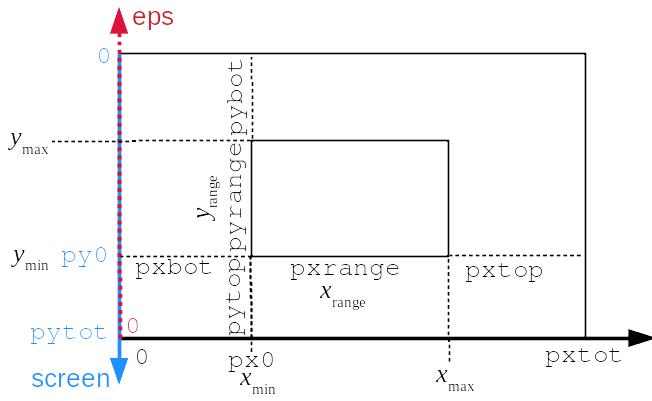
\includegraphics[scale=0.8]{vplotcoor.png}
\caption{\label{vprange}\ouni{../com/vgraph} coordinates}
\end{figure}



\oguifh{Plot area}{../com/asfigure}
This frame contains a paintbox (i.e. a plot area) to be embedded in a GUI and a \unico{Vplot} object using the paintbox canvas. 
Added functionality includes handles to edit fields in order to translate mouse actions to numbers. 

\uses{\ouni{../com/vgraph}, \ouni{../com/asaux}}

\pvar{
\guifco{plot} is a variable of class \unico{Vplot} in \ouni{../com/vgraph}. It is accessible to the parent GUI for direct plotting.

}

\ppro{

\guifco{assignScreen} creates \unico{Vplot} and passes the paintbox canvas in order to plot on the screen.

\guifco{forceMargin*} set fixed margins for the plot and supresses auto-scaling by subsequent calls to \guifco{Init} or \prcod{vgraph}{Axis}.

\guifco{Init} starts the plot. Inputs are the horizontal and vertical ranges, flags where to put axes and the descriptions of the axes, a flag to mark the origin and another flag to adjust the aspect ratio (i.e. increasing the smaller of the two ranges until the units are of same size, see \prcod{vgraph}{AdjustAspectRatio}).

\guifco{SetSize} to be called from the parent GUI on resizing is used to change the size of this frame.

\guifco{PassEditHandle*} accepts the handle to a \code{TEdit} field in order to link it to the mouse position inside this frame.

\guifco{PassFormHandle} accepts a handle to the parent GUI. \todo{(?)}

\guifco{GetRange} returns the range of a rectangular region in physical coordinates, which has been marked by dragging the mouse inside the plot.

\guifco{UnfreezeEdit} frees the edit fields again, when it had been frozen by an Mouse/up event (see below).
}


\act{
\evcodxf{plot area}{pMouseDown,pMouseMove,pMouseUp} handles mouse events inside the plot area.
When edit fields are linked, the physical coordinates of the plot are displayed in the fields while moving the mouse. On releasing the mouse, the edit field freezes, i.e. saves the last data and changes its color.
This is used in \ogui{opatrackps} %{PassEditHandle..} 
to see the particle coordinates corresponding to the cursor position. \\
When the mouse is dragged, the region between mouse down and up is used to rescale the plot area. This is used to zoom in in \ogui{opageometry}~-- \todo{This works in Windows but not in Linux, probably due to different event handling~-- not yet understood.}

\evcodxf{plot area}{pDblClick} grabs the plot image to the Clipboard on double-clicking the mouse.
}



\ounih{Contour plot calculation}{../com/conrect}

\desc{This contour plot calculation is taken from \cite{CONRECT} with minor adaptations. Given a 2D array of rectangular gridded data it returns an array of contour lines.}

\uses{none}
\pvar{
\unico{Con...} are a set of types to store the data. \unico{ConLinesType} contains points of a straight line belonging to an contour of height index \unico{ih}, and \unico{ConLinesArray} is an array of these.
}
\ppro{
\unico{Conrec} is the only procedure, calculating the contours.}

\ounih{Utilities}{../com/asaux}

\desc{This unit is a collection of "little helpers" for formatting numbers and strings, for defining colors etc. Some of this functions may be obsolete meanwhile, since newer versions of Lazarus and Pascal may include corresponding functions.
Procedures are short and probably self-explaining. Not all of them are used in OPA (the \code{../com} folder units are used by several programs).}

\uses{none}

\section{\label{secedit}Lattice I/O and Edit} 

\ounih{Lattice files}{latfilelib}

\desc{Lattice data are read from and saved to files called \code{*.opa}. Reading a file copies its content into a linked list of characters (basically a long string) in \grcod{opamenu}{ReadFile}.

There is an option to read additional files of magnet calibrations and allocations (i.e. real magnet types and names associated with the element), in order to prepare data for the machine control system.

Files from other beam dynamics programs can be read and written, however, this includes only the basic parameters and may require some manual editing to make these files work. This includes Tracy-2 or -3 files \code{*.lat}, Elegant files \code{*.ele,*.lte}, MAD files \code{*.mad} and MAD sequence files \code{*.seq}.
}

\uses{\ouni{globlib}, \ouni{mathlib}, \ouni{../com/asaux}}

\ppro{
\unico{Latread} evaluates the character list of type \unico{TextBuffer}: comments, enclosed by \{ \} brackets, are skipped. An input line is terminated by a semicolon (;), its length is unlimited and it may break over several lines in the lattice file.  Input lines are evaluated by searching first for a colon (:) which identfies an element or segment, or, if not found, a variable.

A variable input line contains a name, an equal sign ($=$) and a value or an expression.
Reserved variables are found searching for the names TITLE, ALLOCATION, CALIBRATION (containing a title of the lattice and the names of optional allocation and calibration files), and by searching in the list of keywords \unico{globkeyw} containing ENERGY and other global parameters. Other names not matching these keywords are considered as user-defined variables.

An element or segment input line contains a name, the colon (:) and a comma-separated list of tokens.

An element is recognized if the colon is followed by a valid element type name in list \unico{elemkeyw} (which is based on \unico{ElemName} in \ouni{globlib}). Then the tokens are expected to contain each a parameter identifier, an equal sign ($=$) and a value or expression. There are many parameters for the different element types. The element is created and the values are assigned.

For a segment the tokens are names of elements or segments, both are  assigned to a linked list of type \unico{AbstractEleType} as defined in \ouni{globlib}.

If names of allocation or calibration files were given, these files are read now.

Finally, the lattice is built from the last segment calling \prcod{globlib}{MakeLattice}.\\


\unico{LatReadCom} is called after LatRead and searches the lattice string for a pair of tokens \code{\{com} and \code{com\}} to save the text between. All other comments contained in the lattice and enclosed in \{ \} brackets only are not saved.\\

\unico{ReadAllocation} and \unico{ReadCalibration} read additional optional files containing lists of magnet types and real names and the magnet calibrations in order to calculate the magnet currents in \guico{opacurrents}. 
An example for SLS is found at \url{https://ados.web.psi.ch/slsdesc/optic/magnets.html}. 

The \unico{ElementType} in \ouni{globlib} contains a pointer to a linked list of \unico{NameListType},  which contains real names of elements, name of power supply, i.e. control channel, polarity etc. \\


\unico{lteconvert}, \unico{madconvert} and \unico{madseqconvert} try to make Elegant \code{*.lte} and MAD \code{*.mad} and \code{*.seq} files understandable for OPA. They work on the \unico{TextBuffer} string by exchanging keywords and inserting conversion factors without analyzing the lattice itself. This is then done by a subsequent call to \unico{LatRead}. Tracy \code{*.lat} and Elegant \code{*.ele} files can be digested directly by \unico{LatRead}.\\

\unico{WriteLattice} accepts a variable \unico{mode} of value \code{0..5} to write an OPA, Tracy-2, Elegant, MAD-X, BMAD or Tracy-3 file. \unico{mode} \code{6} writes an OPA-file with all arithmetic expressions expanded into numbers.

Different beam dynamics codes use different units (e.g. degrees or radians) and different definitions of magnet order and strength. Only OPA, Elegant and Tracy-3 handle correctly nested inversions of segments to implement an asymmetric element (e.g. dipole with different entry and exit edge angles) correctly in the lattice. Export to the other programs requires to create and insert inverted segments (prefix \code{I\_}) for all segments containing asymmetric elements.

All  programs mentioned above allow arithmetic expressions instead of plain values for element parameters. However, unlike the others, Elegant uses inverse Polish notation, which is not included here, therefore expressions are expanded, i.e. resolved to values, for Elegant.

Further export of data is straightforward: first variables, then elements, then segments. The complete lattice file is returned as one long string.
}

\todo{Type \unico{TextBuffer} is a linked list of characters and has historical origin. It could be replaced by a long string, which would be much simpler.}

\oguih{Text Editor}{opatexteditor} 
\desc{A simple Notepad-like text editor to edit the lattice file. The content of the edit window is one variable of type \unico{textbuffer}, i.e. the editor "does not know" what the content means. At exit or when a test is requested, \prcod{latfilelib}{LatRead} is used to analyze the lattice.}

\uses{\ouni{globlib}, \ouni{latfilelib}}

\ppro{
\guico{Init} called from \ogui{opamenu} accepts a handle to the drop down list of segments in order to change its content when segments are created or deleted.

\guico{LoadLattice} called from \ogui{opamenu} calls \prcod{latfilelib}{WriteLattice} to write the lattice file into the text window \guico{EdtWin}. Then the text window is copied into a text buffer to save its content.
}

\act{
\evcodx{text window}{disableOKBut} disables the \ofld{OK} button when text is changed. No other action is done on text input.

\evcod{Test}{filetest} performs a test of the input by calling \prcod{latfilelib}{LatRead}. Before, the input is copied into a buffer, then, by calling \prcod{globlib}{PassErrLogHandle}, the output from \unico{LatRead} is redirected from the \ogui{opamenu} main log window to the local error log window \guico{myerrlog}, because the main GUI may be covered by the text editor GUI. If the test is successful, the \ofld{OK} button is enabled. Then the handle for output is set back to the main GUI.


\evcod{OK}{fileget} reads the lattice in the same way, now knowing that the input is a valid lattice, and exits. At Exit, the segment drop down list in the mnain GUI is set to the last segment, from which the lattice was built by \prcod{latfilelib}{LatRead}.

\evcod{Cancel}{fileRestore} ignores the text window, reads the lattice from the buffer as saved at \guico{Init} and exits.

}

\todo{Nowadays better text editors may be available, which include colored mark-up, auto-complete options and real time checks.}

\oguih{Interactive Editor}{opaeditor}

The "OPA Editor" allows to create elements and compose a lattice without knowing element type names and lattice file syntax. It is more suitable for beginners, while the text editor may be more convenient for experienced users.

The GUI displays two lists, one for variables and elements, the other one for segments. In addition some global parameters like beam energy and default magnet aperture may be set.

\uses{\ouni{globlib}, \ogui{oelecreate}, \ogui{oeleedit}, \ogui{osegedit}, \ouni{../com/asaux}}

\ppro{
\guico{Init} called from \ogui{opamenu} accepts a handle to the drop down list of segments in order to change its content when segments are created or deleted. Init is also called internally to update the list contents.
}

\act{
\evcodx{Element list}{ListBoxEClick}: if the first line of the list is licked, the object \guico{EditElemCreate} of class \ogui{oelecreate} is initialized by passing handles to this list and to the \ogui{osegedit} object for editing segments. If another line of the list is clicked then object \guico{EditElemSet} of class \ogui{oeleedit} is intitalized by calling two different procedures depending on if the clicked item represents a variable or an element, and a handle to this list is passed.

\evcodx{Segment List}{ListBoxSClick} initializes object \guico{EditSegSet} of class \ogui{osegedit} by passing a handle to this list.

\evcod{Beam energy}{EditGloEKeyPress}, \evcodx{aperture fields}{EditA*KeyPress},\\ \evcod{Magnet pole radius}{EdrrefKeyPress} are edit fields to accept values for beam energy, for element default apertures, and for default magnet pole inscribed radius.

\ofldx{Comment window} (no event) text window \guico{MemCom} accepts a comment, which will be saved in the lattice file between the \code{\{com...com\}} tokens.

\evcod{Invert all dipole polarities}{ButDipInv} inverts all dipole polarities.

\evcod{Expand undulators}{ButExpUndClick} expands an undulator into a series of dipoles and drift spaces creating the elements and re-defining the undulator as segment. Usually undulator is a basic element, and the series of dipoles and drifts is executed internally and not visible to the user.

\evcod{Set all apertures}{ButAllAperClick} sets all apertures to the values given in the \guico{EditAx}, \guico{EditAy} fields thus overwriting individual element settings. 

\ofld{Set all (not only if larger)} (no event) if checkbox \guico{ChkAll} is checked, apertures of all elements are set, otherwise only those which have a larger aperture than the values in the fields.

\ofld{Invert rotations in inverted segments} (no event): If  checkbox \guico{ChkGloRi} is ticked or not defines if a beam rotation is inverted (like an asymmetric elements) or not when a segment containing the rotations is  inverted. A corresponding flag \unico{glob.rot\_inv} is set and saved in the lattice file.

\evcod{Exit}{ButExit} saves data, updates the segment drop down list in \ogui{opamenu} and closes the GUI.
}


\oguih{Element Creator}{oelecreate} 

\desc{This small GUI pops up, when \code{new entry} is clicked in the \ouni{opaeditor} elements and variables list. A new element or variable is created after selecting its type and giving it a name. Then the GUI is closed and the \ogui{oeleedit} GUI pops up.}

\uses{\ouni{globlib}, \ogui{oeleedit}, \ogui{osegedit} }   
\ppro{
\guico{Init} accepts handles to the \ogui{opaeditor} elements list and to the segment editor \ouni{osegedit}, because if an element is created or subsequently modified by \ogui{oeleedit}, the changes should appear in these two GUIs. Then the list of element types is filled with the types defined in \ouni{globlib}.
}

\act{
\evcodx{Kind}{ComETypeChange} selects the type of element from the list.

\evcodx{Name}{EdENameChange} accepts the name of the element.

\evcod{Create}{ButCreClick} tests the input, if a type was defined, if the new entry is a variable or an element, and adds it to the corresponding arrays. Then the GUI closes itself and launches \ogui{oeleedit} using one of the two initialization procedures for variables and elements. If it is an element, in case  the segment editor \ogui{osegedit} is open, it is updated.

\evcod{Cancel}{ButCanClick} closes the GUI doing nothing.
}

\todo{Bug: there is no check for duplicate entries, should be added.}


\oguih{Element Editor}{oeleedit} 

\desc{
Main component of the GUI is a table to edit all parameters of an element or a variable. Some fields may contain algebraic expressions to calculate parameters from variables. This procedure is called in four different ways, for elements and for variables, and from editor or from optics design. For (iron dominated) magnets, a possible pole-profile is plotted.
}

\uses{\ouni{globlib}, \ouni{linoplib}, \oguif{../com/asfigure}, \ouni{../com/asaux}}

\ppro{
\guico{InitE}, \guico{InitEVar}, \guico{InitO},  \guico{InitOVar} are four different initialization procedures, for elements and variables, and for calling from the interactive editor \ogui{opaeditor} or from the linear optics design \ogui{opalinop}. In edit mode, a handle to the element list in \ogui{opamenu} is passed, the element index is taken from the list, and the element to be edited is taken from the original element array \unico{Elem}. In optics mode, the index is given explicity and adresses the \unico{Ella} subset of elements in the lattice, and a handle to the plot window of \ogui{opalinop} is passed to enable an update of the plot when the element is changed. For variables there is only one array \unico{Variable} (The arrays are defined in \ouni{globlib}). \\
Then two private procedures are called, which are common for edit and optics mode, to fill the table with data of the element or variable. For elements several lines are filled depending on the type of element, for variables it is only one line. Some element properties and variables may have a value {\em and} an arithmetic expression (like "A+B"), which is a string for variables and a pointer for elements. If the string is empty or the pointer is \code{nil}, the value is taken in edit mode. In optics mode, the calculated value from the expression is shown too ("2.5 = A+B") for elements. For variables the expression is shown in both modes.\\
If the element is a quadrupole or a bending magnet, the GUI is extended by a plot area of type \oguif{../com/asfigure} to show its pole profile.

\guico{getJelem} just returns the index of the selected element in order to enable \ogui{opalinop} to kill this GUI if the user assigns the element to a knob.
}
\act{

\evcod{Done}{butOKClick} and \evcod{Apply}{butApplyClick} both read the table and update the element. The \ofld{Apply} button is only enabled in optics mode and does not close the GUI in order to view how the change affects the optics.\\ 
The private procedure \guico{SetElem} for updating the element performs several steps:
In edit mode, it reads the name of the element, checks if it already exists, and, if not, if this element is used in segments, and asks, if all these entries should be renamed too. Then, in both modes, the table is read and the values are assigned to the element depending on its type. This includes conversion from convenient input units to internal SI-units. The validity of data is checked, i.e. if values are valid numbers, and if expressions can be executed without error. If everything is ok, then, in edit mode, data are written to the selected element in the \unico{Elem} array and updated in the elements list of the calling \ogui{opamenu} GUI. In optics mode, the element in the \unico{Ella} array is updated, the optics is recalculated calling \prcod{linoplib}{OpticReCalc}, and the plot in the calling \ogui{opalinop} GUI is updated by sending it a \code{repaint} event.\\
For variables, the private procedure \guico{SetVar} performs similar actions: In edit mode it reads the name, checks if it already exists, and, if not, it this variable is used in any expression, and asks if all these entries should be renamed too. Then in both modes, its expression is read from the table. (If the expression can be converted into a valid number, this value is assigned and the expression set to an empty string to identify a primary variable, which is a pure number.) Then, depending on the mode, the \ogui{opamenu} list is updated or the \ogui{opalinop} plot is updated.

\evcod{Cancel}{butCancelClick} does nothing but closing the GUI.

\evcodx{Parameter table}{TabDrawCell} checks if input is a valid number and marks it red in case of error. This is not done in edit mode, since input may be an expression. In optics mode, expressions as input are not editable.

\guico{ppaint} reacts on repaint events for the form and plots the magnet profile, it is activated at initialization.
}


\oguih{Segment Editor}{osegedit}

\desc{
The GUI displays an editable string grid with names of elements and segments, which are marked in color depending on its kind and type. 
}

\uses{\ouni{globlib}, \ouni{../com/asaux}}

\ppro{
\guico{Init} passes a handle to the segment list in \ogui{opaeditor} and loads the abstract element sequence of the segment, which was clicked in the list, into the string grid. If entries contain an inversion flag or a multiplication factors, this is written to the grid cell too. The segment name is written to the \ofldx{Modify segment} name field at top, and its periodicity (replication factor) to the \ofldx{periodicity} field at bottom. If the first line of the segment list was clicked, a new segment is to be created and grid and name edit field stay empty.
}
\act{
\evcodx{Grid}{drawCell} analyzes the content of the cell and assigns a color code for element type, segment or unknown using private procedure \guico{ElemCol\_C}.

\evcodx{Grid}{gridKeyDown} reacts to pressing the CTRL+INSERT or CTRL+DELETE keys on the keyboard by inserting or deleting a grid cell, and shifting up or down the higher cells using private procedure \guico{ShiftCells}.

\evcodx{Modify segment}{EditSegNameChange}: If the name of the segment was changed, the button to create a new segment is enabled.

\evcod{update}{butokClick} and \evcod{create}{butcreClick} call private procedure \guico{SaveSeg} to read the grid cells and edit fields, and to perform several checks before creating or updating the segment:\\
If the grid is empty and the segment is not used by any other segment, then the segment is deleted, otherwise an error message is sent.\\
If the name is invalid or if the name already exists, or if the  segment contains unknown names, error messages are sent.\\
If tests were successful, in case of \ofldx{create} a new segment is appended to the list, in case of \ofldx{update} the existing segment is deleted first by disposing all its abstract element pointers in \prcod{globlib}{ClearSeg}.\\
If an existing segment was renamed, the entry is updated in all others segments. Then, 
the new segment sequence is saved as linked list of abstract elements by \prcod{globlib}{AppendAE}. If the segment was deleted, it is removed from the global \unico{Segm} array and from the \ogui{opaeditor} segment list, else the list is updated. Finally the exit procedure destroys the GUI.

\evcod{delete}{butdelClick} sets all grid cells to empty strings and performs the delete procedures for an empty segment as described above, and exits.

\evcod{cancel}{butcanClick} does nothing but exit.
}

\section{\label{seclino}Linear Optics}

\oguih{Linear optics design}{opalinop} 

\desc{This is the main GUI for linear optics development. It contains a plot window to show optical functions along the lattice, a table to display beam parameter results, a couple of knobs to be assigned to elements and several buttons for various options and for changing the display. Unlike all other GUIs, the plot window here is not based on \oguif{../com/asfigure}, because it is too complex. All the beam dynamics calculations are done by \ouni{linoplib}.}

\uses{\oguif{knobframe}, \ogui{ostartmenu}, \ogui{otunematrix}, \ogui{owriteomrk},\ogui{obetenvmag}, \ogui{omatching}, \ouni{linoplib}, \ogui{opatunediag}, \ogui{oeleedit}, \ouni{globlib}, \ouni{mathlib}, \ouni{../com/vgraph}, \ouni{../com/asaux}} 

\ppro{
\guico{Init} is called from \ogui{opamenu} passing a handle to a tune diagram as defined in \ogui{opatunediag}, which is further passed to \ouni{linoplib}. A \unico{Vplot} object as defined in \ouni{../com/vgraph} is created, the corresponding variable for the plot window named \unico{vp}, however, is defined in \ouni{linoplib}, where the calculations take place. A handle to the parameter table \guico{tab} is also passed to \ouni{linoplib}. Then some inital values are set for various data.\\
If the lattice contains variables, copies of their values are saved, and all elements containing expressions are evaluated to check if the variables are used or not in the lattice. For each variable in use, a label is created underneath the plot window. If it is a primary variable (i.e. a number), which can be edited, the label is yellow, if it is a dependant variable (i.e. an expression) the label is pale yellow.\\
Finally the GUI is resized based on saved user settings. This causes a repaint event of the plot area:
}

\act{
\evcodx{GUI resize}{FormResize} reacts to a resize of the GUI by the user or by the \guico{Init} procedure. The GUI is resized by reserving space for buttons etc. and adjusting plot area, parameter table and labels for the variables to left over space.
Then as many knobs as fit into the GUI are created. these knobs of class 
\guifco{TKnob} are defined in   Since a knob may affect the values of other knobs (in case it will be assigned to a variable), each knob receives handles to all other knob calling public procedure \guifco{BrotherHandles} of \oguif{knobframe}. If the GUI was shrinked, knobs which don't fit in anymore are freed (i.e. destroyed). Finally, the sizes of all components of the GUI are calculated and set.

\evcodx{plot area}{pwpaint} is not activated by the user but by the system if the \code{paintbox} of the plot area receives a generic \code{repaint} event. This is also done by \ogui{opamenu} after calling \guico{Init}. The event calls the private procedure \guico{MakePlot}, which performs these actions:\\
The plot is initialized, i.e. plotting axes etc. The abscissa is always the longitudinal coordinate along the lattice. Regions representing magnets in the lattice are calculated, plotted and saved to later enable reaction on mouse operations.\\
If \guico{MakePlot} is called for the first time, the start GUI \ogui{ostartmenu} is launched in front of this GUI and will start the first calculation calling \prcod{linoplib}{OpticCalc}. Finally the resulting optical functions are plotted.\\ \todo{This way to launch the start menu is a bit awkward, there may be a better solution.}

\evcodx{plot area}{pwMouseMove} shows the name of an element when hovering over.

\evcodx{plot area}{pwMouseDown, pwMouseUp} drag an element to a knob, if the left mouse button was pressed inside an element region and released inside a knob region. If an element editor \ogui{oeleedit} is open for this element, it is killed. If the element is already connected to another knob, an error message is displayed.\\
If the element is double-clicked, the element editor \ogui{oeleedit} is opened in optics mode, and if there was a connection to a knob, it is released.\\
If the right mouse button is pressed, the optical function values at this location are shown in the lower part of the table \guico{tab}.

\evcodx{variable labels}{varbutMouseDown, varbutMouseUp} perform the corresponding actions to a variable, if the mouse is pressed inside the region of a yellow variable label and released inside a knob region.\\

\evcod{Start}{butStarClick} launches the start GUI \ogui{ostartmenu} again, to change initial parameters of the calculation.

\evcod{PlotMode}{butenvlClick} launches the GUI \ogui{obetenvmag} to select plot of beta functions, envelopes or magnetic fields, and to set some plot parameters.

\evcod{TuneMatrix}{buttuneClick} launches the GUI \ogui{otunematrix} to smoothly adjust the lattice tune within a small range by changing all quadrupoles.

\evcod{Matching}{butmatClick} launches the GUI \ogui{omatching} for automatic matching of optical functions to target values by changing selected knobs (i.e. magnet strengths). Since some magnets may be connected to knobs, a handle to all knobs is passed that the matching program may set them to new values.

\evcod{Write OMK}{butwomkClick} launches a small GUI \ogui{owriteomrk} to select the optics markers to overwrite with the current optics data. (An optics marker is an element to store local optics data, which may be used as a starting point for forward/backward optics calculations.)

\evcod{linear}{butnlinClick} toggles between linear and non-linear calculation by setting the flag \unico{UseSext}, and performs the calculation. The caption of the button is changed to \ofld{nonlinear} in non-linear mode. This option has only an effect on off-axis beams.

\evcod{Kicker OFF}{butkickClick} toggles between kickers on and off by setting the flag \unico{UsePulsed}, and performs the calculation. The caption of the button is changed to \ofld{Kicker ON} if kickers are on.

\evcod{-\textgreater txt}{butdataClick} writes four text files to the working folder, which are named \code{(opa file name)\_data, \_beta, \_mag, \_rad.txt}. They contain the equilibrium beam parameters, the beta functions along the lattice, the magnet field data and another output of beta functions for radiation calculations. 

\evcod{-\textgreater EPS}{butepsClick} exports the plot to an encapsulated postscript file in the workig folder, which is named \code{(opa file name)\_betas, \_envel, \_magfd.eps} depending if betas, envelopes or magnetic fields are shown. 
The procedure \guifco{PS\_start} and \guifco{PS\_stop} are called to switch on and off the postscript mode in \ouni{../com/vgraph}.

\evcod{Exit}{butexitClick} calls \prcod{globlib}{EllaSave} to check for changes of element parameters and to ask the user to save the changes. Then user settings are saved and the GUI is closed.

\evcodx{GUI close}{FormClose} closes the GUI without saving anything.\\

\evcod{\textless--\textgreater}{buzoominClick} zooms into the plot. The six other similar buttons perform similar actions like zoom out, shift left etc.\\ \feature{Internally, elements are subdivided in slices of a maximum length corresponding to one pixel on the screen, so a mini-beta-focus or the dispersion oscillation inside an undular may be resolved!}

\evcod{$\wedge$B(x)}{buyupClick} magnifies vertically the plot of betafunctions or the horizontal envelope, if in envelope mode. In magnetic field plot mode, it has no effect. The four other similar buttons are to shrink the beta plot and to magnify/shrink  the dispersion plot, and to return to automatic scaling.

\evcod{save}{bucsaveClick} saves the plot data to a second set of curves, which then is plotted in a darker color then the current curves in order to have a visual comparison of the changes. These actions take place in \ouni{linoplib}.

\evcod{clear}{bucclearClick} removes the saved curves.

}




\oguifh{Parameter knob}{knobframe} 

\desc{This component provides a knob to control an element parameter considered as strength as defined by \prcod{OPAgloal}{putkval/getkval}. Values may be set by slider or edit field, including range limits and a reset function. As many knobs as fit into the GUIs are dynamically embedded in optics design \ogui{opalinop} and orbit correction \ogui{opaorbit}. Knob actions trigger calculations and plots. Knobs may stay passive and only display the value, if the parameter is an expression controlled by a variable (which may be connected to another knob). Therefore a knob has to know his fellow knobs and to trigger their updates.}

\uses{\ouni{linoplib}, \ouni{globlib}, \ouni{mathlib}, \ouni{../com/asaux}} 
 
\ppro{
\guifco{Init} gives a name using an index provided by the calling GUI (because it numbers the knobs) and initializes the knob as being not yet connected.

\guifco{SetSize} adjusts the knob to the size as given by the calling GUI. There is a minimum and maximum size, within this range the knob component is "elastic". If the range is exceeded, the number of knobs is adjusted by the parent GUI.

\guifco{Brotherhandles} accepts handles to the other knobs in the GUI.

\guifco{Load} and \guifco{LoadVar} connect the knob to an element or variable, accepting as input the index of the element or variable and a handle to the plot window of the parent GUI. If the parameter is an expression, the knob stays in passive mode, if it is a number, the knob is active. Element/variable name is written to the knob and range limits are set to values of same magnitude like the current value. The current value is saved. The element/variable is tagged in order to not connect it twice.

\guifco{UnLoad} removes the element/variable tags and sets back all captions to the initial status of being not connected.

\guifco{KUpdate} sets the knob to a new value by adjusting edit field and slider, and, if exceeded, also the range limits. If the knob was updated manually, private procedure \guifco{Action} is called to trigger calculations and plots and, if needed, to update the other knobs. If the knob is updated in this way from another plot, no further action takes place.\\
If the knbos are components of \ogui{opalinop} the {\em optics} is re-calculated and the plot is updated depending which mode (betas, envelopes, magnetic field) is set.
If the knob is component of \ogui{opaorbit} the {\em orbit} is re-calculated and the plot is updated.\\
If the knob is connected to a variable, changing it may affect other knobs connected to elements or variables using {\em this} variable in an expression. So all elements' expressions are evaluated to update their values, and, if they are connected to another knob, the \guifco{KUpdate} procedure is called for the {\em other} knob (therefore it's not a circular reference). Of course, this affects only knobs which are in passive mode. \todo{This feature is yet only implemented for optics mode, since in orbit/injection mode no expressions are allowed for corrector magnets and kickers, which are the only elements to be connected. Thus it wasn't needed, however this is an uneccessary restriction.}

\guifco{getella} and \guifco{getvar} return the index of the connected element/variable.
}

\act{
\evcodxf{value field}{editKKeyPress} calls \guifco{KUpdate} to perform actions and adjust the range if the input value exceeds it.

\evcodxf{slider}{sliderScroll} only performs actions, since the slider cannot exceed the given range.

\evcodxf{min/max fields}{editmin/maxKeyPress} as well as \evcodf{\textgreater\textless}{butwidClick} and \evcodf{\textless\textgreater}{butnarClick} adjust the range limits by setting minimum/maximum or widening/narrowing the range, all calling private procedure \guifco{SetKrange}, which sets the small range fields and the slider parameters.

\evcodf{Reset}{butresClick} resets the knob to the value it had when connecting it and performs the actions.

\evcodf{X}{butfreeClick} disconnects the knob calling \guifco{Unload}.
}

\oguih{Start parameters}{ostartmenu} 

\desc{This GUI pops up on initialization of the optics module  \ogui{opalinop} or the orbit/injection module \ogui{opaorbit} (see sec.\ref{secorin}), or when pressing the \ofld{Start} buttons in these modules. The starting conditions for the optics calculation are to be selected, either periodic/symmetric, or forward/backward from start/end of lattice or from one of the optics markers. In case of forward/backward calculation the initial beam parameters may be entered manually, in orbit/injecition mode this is only the orbit. In optics mode it includes also the normal mode beta functions, the dispersions and the elements of the coupling matrix.}

\uses{\ouni{linoplib}, \ouni{globlib}, \ouni{mathlib}, \ouni{../com/asaux}} 

\ppro{
\guico{Load} accepts a number for the mode of operation, which is 0,1,2 for optics, orbit, injection, and a handle to the parent form, which is either \ogui{opalinop} or \ogui{opaorbit}. Depending on the mode radio buttons to select periodic/symmetric or forward/backward options are enabled or disabled (per/symm makes no sense in injection mode). Then the lattice is searched for optics marker and corresponding radio buttons are added to the GUI. In optics mode a check box to perform calculations with or without coupling becomes visible and is checked at start if the lattice contains coupling elements. Finally the panels to enter/edit initial beam parameters are enabled/disabled and filled with data calling the private procedure \guico{set\_pan\_ini}.

\guico{Exit} is called from the parent GUI (\ogui{opalinop} or \ogui{opaorbit}) on exit to close this GUI too if it is still open.
}

\act{
\evcodx{radio buttons}{rbutClick} enables the tables to edit initial parameters depending on the selection of periodic/symmetric or forward/backward calculation, calling the private procedure \guico{set\_pan\_ini}, and enables the buttons to start the calculations.

\evcodx{periodic solution}{rbutperChange}, this radio button has an additional event to hide/unhide the \ofld{flip} check box to start with flipped solution in case of coupling. (Further a button \ofld{pp} appears, which is a temporary test only.)

\evcod{coupling}{chk\_coupChange} hides/unhides the \ofld{flip} check box. 

\evcod{dp/p[\%]$=$}{but\_dppClick} unhides an edit field to enter a value for momentum offset, and a check box to select if one calculation for $Delta p/p$  or three calculations for $0,\pm\Delta p/p$ are to be done.

\evcod{Apply}{butapplyClick} (or \evcod{Close}{butcloClick}) starts the calculation calling private procedure \guico{Go} (and closes this GUI). Before starting the calculation several flages are set depending on the mode (optics with or without coupling, orbit, injection) and the initial conditions. Afterwards, the plot procedures \prcod{linoplib}{OpticCalc} or \prcod{linoplib}{OrbitCalc} are called.

\evcod{Exit}{butexitClick} closes this GUI and the parent GUI (\ogui{opalinop} or \ogui{opaorbit}).

\evcodx{Coupling panel}{ed\_couKeyPress,ed\_couExit} check the input into the edit fields of the coupling matrix (rarely used).
}


\oguih{Optics plot mode selection}{obetenvmag} 

\desc{This GUI is launched by \ogui{opalinop} to select what to show: beta functions (normal mode and/or projected) and dispersions, envelopes with orbit and apertures or magnetic fields. Additional parameters may be set.
}

\uses{\ouni{globlib}, \ouni{mathlib}, \ouni{../com/asaux}} 

\ppro{
\guico{Load} sets GUI components (check boxes, fields etc.) for the current plot settings (explained below) and saves initial settings in order to restore them later.
}

\act{
\evcodx{Beta, Envelope, Mag. field radio buttons}{rmodClick} selects one of the three plot modes (Betas, Envelopes, Magnetic fields), unhides the corresponding panel and hides the two other, and enables options depending on flags: one flag is coupling, another flag is for using equilibrium emittances or input emittances. Further the data table on the right side of \ogui{opalinop} is configured, and table and plot are updated calling procedures \prcod{linoplib}{InitBetaTab,FillBetaTab}. Then the private procedure \prcod{MakePlot} sets plot ranges etc. and calls the corresponding plot procedures \prcod{linoplib}{PlotBeta,EnvPlot,MagPLot}.

\evcod{Apply}{butgoClick} also calls for a new plot and updates the data table.

\evcod{Close}{butcanClick} closes the GUI.\\

\underline{Beta and Dispersion panel:}

\evcod{Fix plot range}{cbxbetamaxClick} enables the fields for max. beta and dispersion if checked. Then, \ofld{Apply} will read the edit fields \ofld{max. betafunction} and \ofld{max.dispersion} and fix the plot range. Otherwise the plot wll auto-scale.

\evcod{normalmode}{chk\_betabChange} and \evcod{projected}{chk\_betxyChange} select to show normal mode and/or projected beta functions. Without coupling this is the same. (The third option \ofld{n.mode one-turn} is only a test.)

\evcod{Dispersion}{rbu\_dspChange}, \evcod{det(C)}{rbu\_cdetChange}, \evcod{Orbit}{rbu\_orbiChange} radio buttons select to show the dispersion functions, the determinant of the coupling matrix or the orbit.\\

\underline{Envelopes panel:}

\evcod{use equilibrium / use input values}{rbuClick} radio buttons select to use equilibrium emittances and energy spread or manual input values for envelope calculation. In the equilibrium case, if the lattice is uncoupled, the field \ofld{emittance coupling} is enabled, otherwise both emittances from the coupled calculation are used. In the input case, three fields \ofld{horizontal emittance}, \ofld{vertical emittance} and \ofld{rms energy spread} are enabled.\\

\underline{Magnet field panel:}

\evcod{Fix plot range}{chk\_bfieldfixClick} enables the fields for min. and max. field if checked. Otherwise the plot wll auto-scale. \ofld{Apply} will read the \ofld{Reference radius} field for pole-tip field calculation, and the two edit fields \ofld{min. B[T]} and \ofld{max.B[T]} to set the plot range. 

}


\oguih{Tune matching}{otunematrix} 

This small GUI launched by \ogui{opalinop} calculates a $2\times 2$ sensitivity matrix how the lattice tunes depend on a scaling factor applied to the two groups of all horizontally and all vertically focusing quads. A new tune may be entered manually, and the inverse of the sensitivity matrix is then used to adjust all quads correspondingly. This procedure converges for small tune changes and was also used in SLS control by exporting the sensitivity matrix to EPICS channels from module \ogui{opacurrents}. The code is simple and may not need further explanation.

\uses{\ouni{linoplib}, \ouni{globlib}, \ouni{mathlib}, \ouni{../com/asaux}} 


\oguih{Optics marker update}{owriteomrk} 
\desc{Optics markers are markers in the lattice which can store beam data (betas etc.) and may be used as starting points for forward/backward calculations by \ogui{ostartmenu}. This GUI establishes a list of all optics markers in the lattice with tick marks and asks if their data should be overwritten with the current optics solution. This may be ambiguos since an optics marker may appear several times in a lattice, so the data refer to the first instance, counting from begin of lattice. The code is simple and may not need further explanation.}

\uses{\ouni{globlib}, \ouni{../com/asaux}} 




\ounih{Lattice calculations}{linoplib} 

\desc{Linear beam optics includes closed orbit finder, periodic solution for coupled and uncoupled lattices, and radiation integrals. 
This unit has handles to the plot areas and tables of the optics and orbit/injection GUIs, \ogui{opalinop} and \ogui{opaorbit}.
Plot routines show beta functions and dispersions, or orbit, envelopes and apertures, or magnetic fields. Lattice and local beam parameters are filled into the tables, and several output files can be printed. 
}


\uses{
 \ouni{elemlib}, \ogui{opatunediag}, \ouni{globlib}, \ouni{mathlib}, \ouni{../com/vgraph}, \ouni{../com/asaux}}

\pvar{
Several variables used by \ogui{opalinop}, \ogui{ostartmenu} etc. are defined in the interface section, i.e. as public, for convenience (i.e. lazyness). Most of them are flags to control the flow. Few of them may require an explanation:

\unico{vp} defines a \guifco{vgraph} object for the optics GUI \ogui{opalinop}, which creates it at start. Later, \ogui{linoplib} itself will plot to \unico{vp}. The orbit/injection GUI \ogui{opaorbit}, however, defines its own plot areas of class \guifco{asfigure} and only gets the data from \ouni{linoplib}. The reason for this different solutions was partly historical, partly due to the higher complexity of the \ogui{opalinop} plot.

\unico{Opval} is a dynamic 2-dimensional array of \code{OpvalType} to save optics parameters after each lattice element and for up to three calculations, e.g. for on- and $\pm$off-momentum.

\unico{Obeam} is a 3-element array to save beam parameters like tunes, emittances etc. for up to three calculations.
}
 
\ppro{
\unico{allocOpval} allocates the array of optics values.

\unico{shiftOpval} shifts up the optics values for one solution the next row in the lattice; this is used to save a solution for comparison with a newer one.

\unico{setTabHandle} receives a handle to the table in \ogui{opalinop} in order to fill in optics results

\unico{setTunePlotHandle} receives a handle to the tune diagram GUI \ogui{opatunediag} in order to plot working points.

\unico{setOrbitHandle} receives a handle to the \ogui{opaorbit} GUI. Actually it is only needed to send it a \code{repaint} event, it will then get and plot the data from \ouni{linoplib}.\\

\underline{Beam dynamics procedures:}

\unico{OptInit} initializes all variables (beta functions, transfer matrix etc.) to be used for the optics calculations.

\unico{Lattel} is the basic procedure for all calculations. It propagates the optical functions through one lattice element. Input is the lattice index and a mode flag telling it what to include in the calculation (integrals, misaligmnents etc). 

\unico{ClosedOrbit} tries to find the fixpoint of the one-turn map, i.e. the closed orbit, by a Newton-Raphson root finder with the {\em local} transfermatrix as Jacobian. It returns a flag to tell if it failed or not. For on-momentum calculation without misalignments, it is trivial and the orbit is on-axis. Else down-feeds from non-linearities affect the local transfermatrix and require some iterations, usually only a few since the method converges quadratically.

\unico{Periodic} tries to find the periodic optics solution, if the closed orbit was found. Depending on coupling it switches to two procedures:

\unico{Flatperiodic} calculates the periodic solution for uncoupled, i.e. flat lattices without coupling elements, where horizontal and vertical dimension can be calculated independently, and vertical dispersion is always zero. The algorithm is described in Klaus Wille's book \cite{kwille}.

\unico{NormalMode} calculates the periodic solution for coupled lattices using the Edward-Teng formalism in the version of Sagan and Rubin and implemented as described in \cite{VZAS}. Section 2 of the "inside OPA" guide \cite{inside} gives a summary. If successful the procedure returns the normal mode beta functions, which have no physical meaning and exist in an uncoupled system (coordinates $a,b$) and the coupling matrix, which translates the normal mode system to the real coordinate system (coordinates $x,y$). It further returns the 4-vector of dispersions and the lattice tunes.

\unico{Symmetric} calculates the symmetric solution with 
$\alpha_x=\alpha_y=D_x'=0$ and works only for uncoupled lattices. It is rarely used and not well tested. The algorithm is also described in \cite{kwille}.

\unico{LinOp} is a {\em private} procedure to propagate the beta functions through the lattice and save the values after each element to the \unico{Opval} array by calling procedure \unico{StoVar}. Usually it would start at the begin of the lattice with initial conditions from the periodic solution or entered manually. But it may also start at an optics marker and propagate forward and backward to end and start of lattice. Care is taken to handle inverted elements and derivatives of optical parameter and to sum up integrals correctly. Depending on the input flag \code{latmode} only the beta functions and dispersions are calculated or chromaticities and radiation integrals are calculated too by passing the flag to the \unico{Lattel} routine, which passes it further to the element propagation routines.

\unico{OpticCalc} performs the full linear optics calculation by calling \unico{ClosedOrbit}, \unico{Periodic} and \unico{LinOp}. Afterwards, the working point is plotted to the tune diagram (in case of periodic solution only) and the table in \ogui{opalinop} is filled calling procedures \unico{FillBeamTab} and \unico{FillBetaTab}. \\
\todo{The code is a bit messy due to the different cases it has to handle~-- periodic/symmetric solution or forward/backward from an optics marker, how many calculations to do, on- or off-momentum.} 

\unico{OrbitCalc} is a simplified version of \unico{OpticCalc} used by \ogui{opaorbit} for calculation of orbit only. An additional feature is the ability to do several turns which is useful in injection simulation.

\unico{MatchValues} is a function returning an array of type \vrcod{globlib}{MatchFuncType} containing optics values at the begin and end of the lattice, and optionally, at an intermediate point. It is used by \ouni{omatching} for matching optics parameters to target values.\\

\underline{Plot procedures:}

\unico{SliceCalcN} calculates optical functions {\em inside} an element by subdividing it into slices of a length corresponding to one pixel on the screen. Calculations start at each lattice element, where optical functions have been before calculated by \unico{Linop} and saved in the \unico{Opval} array. Elements outside the plot window are skipped, if the user zoomed in to a part of the lattice in \ogui{opalinop}. The variable \vrcod{globlib}{CurvePlot} stores the start and end point and the number of slices and their length, and the optical functions at the slices are saved in the variable \vrcod{globlib}{Curve}, which is a linked list of pointers for storing optical data. Procedure \vrcod{elemlib}{SlicingN} performs these calculation and generates the curve.\\
\feature{It's a unique feature of OPA to display the optical functions at pixel resolution. This allows to export nice plots ready for publication.}

\unico{PlotBeta} displays the beta functions and dispersions. The procedure is lengthy due to the various plot modes as selected in \ogui{obetenvmag}, but in principle it is relatively simple: After setting the ranges, the internal procedure \unico{BetaCurveN} is called to generate the curves calling \unico{SliceCalcN} and to plot them. More than one curve for each function is plotted if a previous curve was saved for comparison, or if a $0,\pm\Delta p/p$ calculations was done.

\unico{PlotEnv} displays the envelope functions. Before, they need to be calculated. Therefore several arrays are created to hold all the data for the orbit and the different contributions to the beam size (from dispersion, from coupling). They are calculated either using input or equilibrium emittances and energy spread as selected in \ogui{obetenvmag}. Also the apertures are plotted calling procedure \unico{PlotApertures}.

\unico{PlotMag} displays the pole-tip field of the magnets. No slicing is done since the magnets have no longitudinal variation of the fields (longitudinal gradient bends are approximated by a stack of dipoles). In case of the solenoid, the longitudinal field is shown. For combined function magnets only dipole and quadrupole field is used for pole-tip field calculation. The reference radius as set in \ogui{obetenvmag} is assumed to be the same for all magnets.

\unico{PlotOrbit} is used by the orbit \& injection GUI \ogui{opaorbit} only, whereas the other plot procedures are only used by the optics GUI \ogui{opalinop}. \ogui{opaorbit} does the plotting by itself, so this plot procedure just sends a repaint event to its formhandle.\\

\underline{Output}

\unico{FillBeamTab} and \unico{FillBetaTab} write equilibrium beam parameters and beta functions at the location which was right-clicked (see above: \ogui{opalinop} action \evcodx{plot area}{pwMouseDown}) to the table on the right side of \ogui{opalinop}. In envelope mode, beam sizes, correlations and beam tilt angles are calculated and displayed. 

\unico{Print\dots} These procedures print various data to files: lattice data in text or html format, beta functoins curves, magnet and radiation data.
}

\ounih{Element calculations}{elemlib} 

\desc{This unit contains the procedures to propagate optical parameters through the different elements in the lattice. They all receive the variable \unico{mode} telling them what to include in the calculation, by evaluating \prcod{globlib}{switch}. Most elements receive the varialbe \unico{idir} to set forward or reverse orientation of the element (for example important for a dipole with different edge angles). All other parameters are explained in the user guide \cite{userguide}. 
The flags \unico{UseSext,UsePulsed} in \ouni{globlib} switch on/off non-linearities and kickers. Coupled calculation is selected by the element procedures. Another set of procedures performs the sliced calculations for thick elements to provide data in pixel-resolution for a nice display. 
}

\uses{\ouni{globlib}, \ouni{mathlib}}

\subsubsection*{Procedures}

This section tries to list the procedures in a logical order (not as they apppear in the file) for best understanding. Some are public, to be called by \ouni{linoplib}, others are private and commented out in the \code{INTERFACE} section of the file.\\

\underline{Beam propagation}

\unico{Propagate} receives the transfermatrix of an element and a flag on coupling to propagate the optical functions from start to end of the element using two procedures:

\unico{MCC\_prop} proceeds {\em with} coupling to propagate the normal mode beta functions and the coupling matrix. In the beginning, on- and off-diagonal $2\times 2$ submatrices are extracted from the $5\times 5$ transfer matrix, and a test is done, if a mode flip will happen. Then follows a longer section to handle a possible mode flip. \todo{This section is partly experimental and needs further elaboration. It does not work correctly with regard to tunes and integrals in all cases.} At the end follows the normal case which works reliably with weak coupling. Phase advances are calculated by procedure \unico{PhaseAdvance} and added to the ring tunes, and the dispersion vector is propagated, which always works.

\unico{MBD\_prop} proceeds {\em without} coupling where the transfer matrix is known to be block-diagonal. Nevertheless, possible coupling in the beam has to be propagated too by transforming the coupling matrix, which may have non-zero elements in this case. 

\unico{PropForward} just copies optics parameters after propagation (suffix 2) to parameters before propagation (suffix 1) in order to continue with the next element.

\unico{PhaseAdvance} calculates the block-diagonal normalized normal mode matrix from the local beta functions using the transformation matrix from function \unico{CirMat}, and extracts the phase advances from the traces of the sub-matrices. \unico{getdTune} is a simplified version for a transfer matrix which is known to be block-diagonal.

\unico{GetBeta12} calculates the projections of the normal mode beta functions to the physical beta functions.

\unico{Pathlength} calculates the path length by estimating the second order matrix elements as defined in TRANSPORT (see comment in code for details).\\

\underline{The elements}

The \unico{\dots\_Matrix} functions return $5\times 5$ transfer matrices of the basic linear elements. Since OPA does not include longitudinal dynamics, there are no rows and columns for phase/time and the 55-element is always 1. The fifth column of the matrix contains the dispersion production vector. Drift space, quadrupole, sector magnet and edge kick have block-diagonal matrices, i.e. they don't couple. Coupling elements are the explicit rotation and the solenoid. The Bending magnet matrix is a sector matrix sandwiched between edge kicks. The matrix functions are called by the element procedures. 
OPA knows 17 different elements as listed at the very beginning of \ouni{globlib}:

There are no procedures for markers, optics markers and photon beam markers, because they don't act on beam dynamics. There is a placeholder procedure \unico{Monitor} for beam position monitors but it does nothing. The septum element~--as seen from the stored beam~-- is handled as a drift space in beam dynamics.

\unico{DriftSpace}, \unico{Quadrupole} and \unico{Bending} are the standard linear lattice elements. Actually \unico{Bending} switches to \unico{Quadrupole} if the bend angle is zero, and \unico{Quadrupole} switches to \unico{Driftspace} if the gradient is zero. 
So \unico{Bending} is the most complex procedure and should be explained in some detail. It performs the following steps: at first the magnet is misaliged, if misalignments were requested, then a rotation is applied if the magnet is tilted. Depending on the direction of the magnet, the edge angles are interchanged and the edge kick matrices are calculated. Then the beam (i.e. the optical functions) is propagated through the entry edge because the values at the beginning of the sector are needed to estimate the phase advance inside the sector (procedure \unico{getdtune}) in order to set the right number of points for numerical evaluation of the radiation integrals. Before doing so, the complete bending magnet matrix including entry edge, sector and exit edge is calculated twice, first on-axis (\code{TM0}) as needed for the closed orbit finder, then off-axis (\code{TM}) to include dispersion downfeeds for the integrals. If radiation integrals or chromaticities are requested, the sector is split in a number of slices, the beam is propagated step-wise, and the integrals are obtained by Simpson's rule (see section 3 in \cite{inside} for details, also for the other elements). Finally, the beam is propagated through the complete bending magnet, and rotation and misalignments are undone at exit. \unico{Quadrupole} contains a simplified version of this algorithm, but including radiation integrals too, since there may be off-axis contributions.

\unico{Combined} is a bending magnet which also has a sextupole component. It is modelled as a series of bending magnets with thin sextupole kicks between. Having both \unico{Combined} and \unico{Bending} has historical reasons, and maintaining both is for backward compatibility, but in principole they could be united.

\unico{Undulator} contains a loop over rectangular bends and drift spaces, where the parameters of these sub-elements are set by the procedure \unico{UnduFacs}. For the radiation integrals a simplified algorithm using averages is applied since the bends inside the array are small.

\unico{Solenoid} is a simplified treatment of the solenoid providing beam rotation and focusing in both planes. Note, that the transverse vector potential components of the solenoid are not taken into account, also contributions to chromaticity and radiation are not considered.

\unico{Rotation} is an explicit beam rotation. It's rarely used, because rotated elements like skew quadrupoles are rather set up by passing a rotation angle to the corresponding element procedure. Then the element matrix internally is sandwiched between the rotation and its inverse.

\unico{ThinSextupole} and \unico{Multipole} are thin multipole kicks~-- basically, a sextupole is just a multipole of order 3, but the dedicated procedure executes faster. The procedures apply a non-linear kick to the orbit and a transfer matrix to the optics for off-axis gradient downfeed. (For order 2, quadrupole, there is a gradient on-axis too.) Contributions to radiation integrals are usually negligible and therefore not included. The \unico{Multipole} procedure uses explicit expressions up to octupole (order $n=4$). For higher orders the general complex expression is evaluated (see comment in code). A vertical offset of the beam requires coupled treatment due to skew quad down-feed.

\unico{Sextupole} is a thick sextupole, internally modelled as a series of drifts and thin sextupole kicks as the most simple second order symplectic integrator. A corresponding procedure for a thick general multipole does not exist yet.

\unico{Kicker} is a time-dependent thick multipole. Parameters delay and period (of half sine bump) and the time of flight from the start of the lattice define the kick strength applied. Like the thick sextupole, the kicker is subdivided in a series of drifts and thin kicks. The transverse shape of the kick can be selected to be of multipole or  sine shape (BESSY type NLK). Note that for the NLK, the kicks are only correct in the midplane ($y=0$).

\unico{HCorr} and \unico{VCorr} are correctors, i.e. weak dipoles which just give a kick to the orbit and to the dispersion function without further effect on the beam optics.\\

\underline{Slicing}

The \unico{SliceSet} function calculates the number of slices for the optical functions inside an element to be displayed in one-pixel resolution on the screen. The record \vrcod{globlib}{CurvePlot} contains a field \unico{slice} for the length of the slice in physical coordinates, i.e. in meters, calculated by \prcod{opalinop}{Zoom}. The \unico{SliceSet} function checks if the element is outside, partially inside or completey inside the current plot window, or if the plot window is completely inside the element. It writes start and end position inside the element and the number and length of slices to the \unico{CurvePlot} record and returns \code{true} if at least a part of the element will be visible in the plot area.

\unico{SlicingN} receives transfer matrices \unico{msl} for a slice, \unico{mof} for the invisible part of the element left of the plot window, and \unico{min} and \unico{mex} for edge focusing at entry and exit of the element (applies to bends only). Additional matrices \unico{mof0,msl0} without dispersion down-feeds are supplied to show both orbit and dispersion functions correctly. The procedure further receives the optics values at the entry to the element, because these are known from the previous run of \prcod{linoplib}{Lattel}. Then optical parameters at the slices are calculateed using a simplified propagation procedure and the results are appended to the \vrcod{globlib}{Curve} variable for later plotting by \ouni{linoplib}. Finally the optics value at the end of the calculation (which may be still inside the element) overwrite the optics values from input.

\unico{SkippingN} is only needed for undulators, which are modelled as a loop over drifts and bends, and where several of these basic elements may be left of the plot window. The optics values are propagated through these invisible basic elements to get the correct initial values at the first partially visible undulator pole. \feature{In this wasy it is possible to zoom into an undulator and see the dispersion oscillation!}

The \unico{Slice(Drift,Quad,Sol,Bend)N} procedures call \unico{SliceSet} and calculate the required transfermatrices for \unico{SlicingN} and \unico{SkippingN}.

\unico{SliceUnduN} loops over bends and drifts of the magnet array if at least a part of the undulator is inside the plot window.

\unico{SextKickN} is a simplified version of \unico{ThinSextupole} to propagate optics values through a sextupole kick.

\unico{SliceSextN} and \unico{SliceCombN} make use of \unico{SextKickN} because they model thick sextupole and combined function magnet as loop over drifts or bends with sextupole kicks between.



\oguih{Linar matching}{omatching} 

\desc{Matching implements a linear equation solver based on LU decomposition for the linear optics. For historical reasons, it does not use the solver in \prcod{mathlib}{LUDCMP,LUBKSB} but the algorithm was explicitly coded in the 1980's by Klaus Wille (procedure \guico{Step}) , and is documented in his book~\cite{kwille}. Matching is done from a start point to an end point in the lattice. The lattice tunes and optics functions at an additional intermediate point may be included too.  After selecting these options, a list of available knobs is established. Then the user selects the constraints, i.e. the optics parameters at end (and intermediate) point, sets the target values and selects at least the same number of knobs (e.g. quadrupole strength, variable etc.) from the list. The solver proceeds using the square matrix of most sensitive knobs, which is recalculated after each step to take into account non-linearities. If successful, the method converges quadratically, if not it returns messages, what went wrong (procedure \guico{Term}). Reduced step size can be set for slower but more robust convergence. It is possible to run a scan over some range of target values. \\
There are three panels at the right side of the GUI, one for the knobs, one for the matching process and one for parameter scans. Only one of them is visible at a time.\\
\todo{The algorithm itself with catches for errors as implemented over the years, is quite robust and could be used further in principle. However, nowadays better and well proven solvers may be available, which also include limit ranges for the knobs. Further, the present procedure is restricted to uncoupled lattices and to only one intermediate point besides start and end of matching, which sometimes is a nuisance. The present GUI is well conistent (how options are enabled etc.) but its rigid structure makes extensions cumbersome. It should be re-organized for example using tabs.}\\
Expecting a rewrite of this module in future, only a brief summary of the most important actions will be given here.}

\uses{\ouni{linoplib}, \oguif{knobframe}, \ogui{omatchscan}, \ouni{globlib},  \oguif{../com/asfigure}, \ouni{../com/asaux}} 

\ppro{
\guico{Load} initializes the GUI. It receives handles to the \code{PaintBox} plot window and to the array of \oguif{knobframe} knobs in \ogui{opalinop} in order to be able to set the knobs to new values and to show the new optical functions after matching. Then it searches for optis markers, which may be used as start, end or intermediate point for matching, and adds them to the \guico{ini/mat/midpoint} pulldown lists. Several user settings are restored from a previous session, since often the same matching scenario is used again.
}

\act{
\evcod{starting,matching,intermediate}{(ini,mat,mid)pointChange} call the private procedure \guico{knoblist} to establishes the list of available knobs after selecting the start, end (and optionally intermediate) points for matching. For each knob a named check box is created.

\evcod{Optics parameter check boxes}{cselClick} and \evcod{Knob check boxes}{knobSelect} build the lists of constraints and knobs and set the \ofld{Go} button if there are at least as many knobs as constraints.

\evcod{incl.bends}{cbxIncBendsClick} includes bending magnets in the knob list, because often they are not used, so the panel is less crowded if they are not shown.

\evcod{Go}{gobutClick} hides the knob panel\guico{panknobs} and shows the matching panel \guico{panmat} with a grid of knob values. Then the iteration starts until the procedure \guico{Step} returns \code{true} because it terminated with success or failure, or the user stopped the iteration pressing \evcod{Abort}{bustopClick}. The last option requires the Pascal procedure \code{Application.ProcessMessages}, which reacts to GUI events, to be called inside the loop. After termination buttons become active to show the result in \ogui{opalinop}, to accept the new values, to reset to initial values or to retry the calculation (for example with reduced step size to be entered in the \ofld{Fraction [\%]} field, in case of bad convergence.)

\evcod{Show}{butShowClick} actually only hides the \ogui{omatching} GUI (which is modal!) to  uncover the \ogui{opalinop} GUI which is behind and shows the current optical functions anyway.

\evcod{Accept}{butaccClick} saves the settings and closes \ogui{omatching}.

\evcod{Reset}{butaccresClick} restores the old knob values, recalculates the optics, saves the scenario and closes the GUI.

\evcod{Retry}{butrtyClick} restores the old knob values and sets up for a new iteration.

\evcod{Scan}{ScanClick} prepares for a parameter scan, i.e. a series of matching iterations for a range of target values. For this purpose, the scan panel \guico{panfig} becomes visible, the modal GUI \ogui{omatchscan} is launched to enter range parameters, and then the matching series are started, the results are saved and plotted eventually. The \ofld{$<,>$} buttons under the plot window allow to toggle between displays for the knobs and functions.
}


\oguih{Parameter scan}{omatchscan}

\desc{This very simple modal GUI is launched by \evcod{omatching}{ScanClick} that the user may enter the range for a parameter scan. At exit it writes the data to the variable \vrcod{linoplib}{ScanPar}, from where \ogui{omatching} takes them to perform the scan.}

\uses{\ouni{linoplib}, \ouni{globlib}, \ouni{../com/asaux}} 


\oguih{Tune diagram}{opatunediag}

\desc{The tune diagram GUI is created at start of OPA already and provides the variable \guico{tuneplot}, which is passed in the initialization procedures of the modules using it: \ogui{opalinop} shows the working point, i.e. the tunes of a periodic solution. \ogui{opamomentum} shows the variation of tunes with momentum. \ogui{opachroma} shows an analytical estimate of the tune footprint. And \ogui{opatrackps} shows the amplitude dependent tune variation. In the background always shown is the web of resonance lines.}

\uses{\ouni{globlib}, \oguif{../com/asfigure}, \ouni{../com/asaux}}

\ppro{
\guico{Diagram} makes the tune diagram visible if a periodic solution exists. Input is the point in tune space where to center the diagram.  The resonance lines inside the visible tune region up to the selected order are calculated by private procedure \unico{getLines} and characterized as regular, skew, non-systematic.  The periodicity of the lattice is stored in \vrcod{globlib}{NPer} and determines the selection of systematic resonances. 

\guico{AddTunePoint} adds a tune point to the diagram. If the input flag \guico{connect} is \code{true} the point is connected to the previous point. The inputs \guico{dpp, dppmax} are used to show off-momentum points in a color range. Used by \ogui{opalinop} and \ogui{opamomentum}.

\guico{AddChromLine} adds a line to show the chromaticity, i.e. the variation of tune with momentum, with chroomaticities up to third order and the momentum range as input. Used by \ogui{opachroma}.

\guico{AddTushPoint} adds points from amplitude dependant tune shift tracking. Input \guico{xmy} controls the color of the points: horizontal, coupled, vertical in blue, purple, red; outside aperture in grey. Used by \ogui{opatrackps}.

\guico{Refresh} clears the diagram from points which had been added.
}
\act{
\evcodx{On create}{FormCreate} sets defaults and restores user settings.

\evcodx{On resize}{FormResize} adjusts the GUI if the user changes its size.

All other actions control the plot: The buttons \ofldx{Order} \ofld{$+$} \ofld{$-$} increase/decrease the maximum resonance order. The \ofld{nsys} and \ofld{skew} check boxes switch on/off non-systematic and skew resonances. The buttons under the plot window are to zoom in/out, to shift the region right/left, up/down and to re-center. \ofld{EPS} exports the diagram.
}

\section{\label{secmomo}Longitudinal optics}
OPA does not contain true longitudinal dynamics, i.e. all calculations are for fixed momentum offset, and tracking proceeds only in 4-D, not in 6-D. There are no cavities and no acceleration.


\oguih{Momentum dependence}{opamomentum}

\desc{This GUI shows optical functions at lattice start and lattice integrals like tunes, emittance etc. for some momentum range. This functionality is the same like performed in \ogui{opalinop}/\ouni{linoplib}: for periodic lattices closed orbit and periodic solution are calculated, then for any lattice, the initial parameters are propagated and the integrals are calculated. The plotted curves of momentum dependent parameters are then fitted by polynomials. In case of pathlength, coefficients are saved internally to be used later in the bucket viewer \ogui{opabucket}.

\todo{For the particular problem to design a non-linear bunch-compressor for an FEL~\cite{nlbuco}, the module once was extended to set target values for polynomial coefficients and allocate non-linear elements to align the polynomial to the target by means of a Powell minimzer. This feature is never used for synchrotrons and storage rings, where the side-effects of this brute force alignment are devastating with regard to non-linear dynamics. Since this extension is irrelevant, improvised and fragile, it should be removed~-- however, this requires some disentangling.}

Therefore only the first part of the GUI is briefly explained here.
}

\uses{\ouni{momentumlib}, \ouni{linoplib}, \ogui{opatunediag}, \ouni{globlib}, \ouni{mathlib}, \oguif{../com/asfigure}, \ouni{../com/asaux}} 

\ppro{
\guico{Start} called from \ogui{opamenu} receives a handle to the tune diagram. Then it assigns handles defined in \ouni{momentumlib} to some of its GUI components to give \ouni{momentumlib} access. Then user settings are restored, and some initialization is done, and the GUI is resized.
}

\act{
\evcodx{On create}{FormCreate} builds the GUI by dynamically creating its components. These include radio button for the 20 different availabe plots as defined in the header of \ouni{momentumlib}. \todo{More components, which have the \guico{panmin} panel as parent, are for the minimizer and to be removed.}

\evcodx{On resize}{FormResize} performs a dynamic resize if the user changes the size of the GUI, distributing evenly the available space.

\evcodx{On paint}{FormPaint} calls \prcod{momentumlib}{MakePlot}\\

\evcod{periodic}{chkPerClick} sets the optics mode to periodic. Of course, a periodic solution may not exist for all values in the momentum range. These failed points will be omitted in the plot.

\evcod{Go}{butGoClick} performs the calculation calling \prcod{momentumlib}{FullCalc}. It also plots the result for the currently selected plotmode, including calculation and display of the fitted polygon. Polynomial coefficients are listed in table \guico{gfit}.

\evcod{Fit}{butFitClick} repeats fit and plot with the selected fit parameters.

\evcod{Units for table}{butfunitClick} toogles between showing the polynomial coefficients in table \guico{gfit} in SI-units or in convenient units as used for the plot annotations.

\evcodx{Radio buttons}{rbClick} sets the plot mode according to the clicked radiobutton and repeats fit and plot. \\

Events not mentioned are either trivial ( e.g. check for valid number in edit fields), or they belong to the (working but irrelevant) Powell minimizer, which is started by the \ofld{optimize} button. 
}


\ounih{Calculations}{momentumlib} 

\desc{This unit contains the physics and plotting for the \ogui{opamomentum} GUI.
}

\uses{\ouni{linoplib}, \ogui{opatunediag}, \ouni{globlib}, \ouni{mathlib}, \oguif{../com/asfigure}, \ouni{../com/asaux}} 

\pvar{
The header contains parameters for the 20 plot modes: color of plot, number format for table, annotation of radio buttons in \ogui{opamomentum} etc. Some plots show two functions, for example horizontal and vertical tune shift. The arrays \unico{ires1,2} control, what to plot. \code{ires2=-1} suppresses the second curve.

\unico{result} is an array of a 20-element array to store the results over the momentum range. The size of the array depends on the number of momentum values to be calculated.

The \unico{...\_HANDLE} variables refer to components of the \guico{opamomentum} GUI.

\unico{res\_funit} contains factors to switch between SI-units and plot units in the polynomial coefficients table.


\todo{All the variables containing \code{"op\_"} or \code{"kn\_"} or \code{"Pen"} in the name belong to the obsolete minimizer.}
}

\ppro{
\unico{Makeplot} shows the selected results. Valid points are plotted as symbols. The internal procedure \unico{fit\_and\_plot} performms a polynomial fit of the requested order over the valid points, shows the fit result as (an) additional line(s) in the plot, and writes the fit coefficients to the table. The internal procedure \unico{plot\_qclines} adds the predictions for the chromaticities from the non-linear optimizer \guico{opachroma} if available, and if tunes were selected for plotting.

\unico{FullCalc} contains the complete calculation:\\
\unico{PreCalc} prepares for the calculation by setting up the momentum values. In case for periodic solution requested, it first checks the on-momentum solution. If successful, the tune diagram \ogui{opatunediag} is launched and the working point is plotted. If chromaticity data are available from a previous run of \guico{opachroma}, they are also shown in the tune diagram as a line. \todo{BUG: diagram appears but no plot, area  stays grey.}\\
\unico{Calculate} loops over the momentum range, calculates the optics parameters and integrals for each momentum value, and stores the results in the \unico{result} array if valid.\\
Afterwards \unico{MakePLot} is called.\\
\unico{PostCalc} finally plots results to the tune diagram if available to show the chromatic tune shift.

\todo{Procedures \unico{CalcPenalty, ShowPenalty, CalcTarg} are obsolete.}

}



\oguih{RF bucket viewer}{opabucket}

\desc{
The RF bucket is calculated based on up to five orders of momentum compaction and RF harmonics as described in \cite{inside}. A contour plot of equipotentials and the separatrix are displayed, and momentum acceptance and the bunch length are estimated.

The coefficients of momentum compaction may be taken over from a previous calculation of momentum dependent optics, \ogui{opamomentum}. The estimates for momentum acceptance and bunch length are saved to be used later in Touschek tracking \ogui{opatracktt}.

For "playing" with the bucket, the viewer may also be used with manual input for cavity voltages and momentum compaction, even without any lattice. Therefore the option is always enabled in \ogui{opamenu}.
}

\uses{\ouni{globlib}, \ouni{mathlib}, \ouni{../com/conrect}, \oguif{../com/asfigure}, \ouni{../com/asaux}} 

\act{
\evcodx{On show}{FormShow} performs all initializations when the GUI becomes visible:  private procedure \guico{Layout} is called to arrange the components (although this GUI does not react to resize by user), user settings are loaded and filled into the edit fields. With this settings, the bucket is calculated immediately and shown by calling private \guico{CalcBucket} and \guico{MakePlot}:

\guico{CalcBucket} performs all the calculations as described in \cite{inside}. This also includes the call to \prcod{../com/concrect}{conrec} to get the equipotential contours, because from these the energy acceptance and bunch length are estimated. However, this requires the central fixpoint to be elliptic (i.e. no overstretched bunches). And bunch length can be estimated only if there is a value for energy spread from a previous optics run.

\guico{MakePlot} just plots the results and writes them to labels in the GUI.

\evcodx{On paint}{FormPaint} just calls \guico{MakePlot} again.

\evcod{Show bucket}{butconClick} calls \guico{CalcBucket} and \guico{MakePlot} again.

\evcod{EPS}{butepsClick} sets mode to postscript export and calls \guico{MakePlot} to write file \code{(lattice name)\_bucket.eps}.

\evcod{mode}{butmodClick} toggles between "lattice" and "play" mode, i.e using momentum compaction coefficients from the lattice or from manual input. 

\evcod{use Lattice}{butcopyClick} copies the lattice coefficients to the edit fields for manual modification in "play" mode. This knob and the \ofld{mode} knob are only visible if an optics calculation had been done before.

\evcod{Exit}{butexClick} saves the user settings and closes the GUI.
}

\section{\label{secnonl}Non-linear Optimization}

The units of this section are linked in a rather complex way as indicated by the \code{uses} declarations, since the main GUI \ogui{opachroma} contains many frames for knobs, \oguif{csexframe}, and for results, \oguif{chamframe}, which affect each other. This required the two small units \ouni{chromreslib}, \ouni{chromreslib}, to pass the handles. \oguif{csexframe} declares use of \ouni{chromreslib}, which declares use of \oguif{chamframe}. Vice versa,
\oguif{chamframe} declares use of \oguif{csexframe} in the implementation section, i.e. at runtime, not in the interface section, to avoid a circular reference. \\
\todo{There may be a better way to declare these dependencies.}

\feature{OPA's non-linear optimizer is a rather useful tool to get a quick optimization of dynamic aperture~-- or to help in understanding why it can't work. Manually playing with the multipoles may give a "feeling" by visualizing the effect on the Hamiltonian modes and the tune footprint, before the automatic minimizer is started. The code executes fast, since all coefficients to sextupole family strengths and products of two families, are calculated only once at start. Multiple periods are realized by a complex factor derived for this purpose~\cite{inside}.}

\oguih{Non-linear optimization panel}{opachroma} 

\desc{
The GUI contains a fixed set of first and second order sextupole Hamiltonian modes and a variable set of knobs connected to non-linear multipole families. These are the sextupoles in first place, which have to maintain corrected chromaticities during optimzation, and optional octupoles and even decapoles. Also sextupole moments in combined function magnets may be included. 

The Hamiltonian modes are scaled by reasonable  betatron amplitudes and momentum range to make them comparable. In addition weight factors are set manually. Optimization may be done by hand "to get a feeling", but usually it is done automatically with frequent user intervention to adjust weights, exclude certain knobs etc. For minimization, the scaled and weighted Hamiltonian modes are summarized to provide a scalar penalty function.

A Powell minimizer is employed to supress first and second order sextupole terms. Second order terms may also be suppressed by an SVD procedure using the octupole families. Both algorithms are based on \cite{numrec} and coded in unit \ouni{mathlib}. Decapoles may only be used manually for third order chromaticity, which is the only third-order effect included.

\todo{Basically, SVD could optimize sextupoles too using the linear system of first order sextupole terms and the linearized (i.e. local tangential) system of second order terms as suggested by Johan Bengtsson and previously implemented in Tracy-2. The mixed approach using Powell and SVD has historical origins but also turned out to perform quite robust.}

Chromaticities up to third order are calculated by numeric differentiation, whereas the other Hamiltonian modes are calculated analytically. A real/complex factor is applied to non-resonant/resonant modes to change the periodicity of the structure~\cite{inside}. 

Besides frames for Hamiltonian modes and multipoles, the GUI contains several edit fields for amplitudes, ranges, periodicity and minimizer settings, many check boxes to select knobs and Hamiltonian modes to be in- or excluded and several buttons to change settings and to control program flow.


\todo{BUG: in the linux version, the frames in the GUI don't update. After touching the GUI (i.e. resize by tiny amount) it works. Not yet understood.}
}


\uses{
\oguif{chamframe}, \oguif{csexframe}, \ouni{chromreslib}, \ouni{chromelelib},  \ouni{chromlib}, \ogui{ochromsvector}, \ogui{opatunediag}, \ouni{globlib}, \ouni{mathlib}, \ouni{../com/asaux}
}

\ppro{
\guico{Start}, called by \ogui{opamenu} receives a handle to the tune diagram \ogui{opatunediag} (to show the prediction of the tune footprint), and then performs many actions:

A fixed number (26) of \oguif{chamframe} frames is installed to show the Hamiltonian modes and change their weights. This requires passing to each one handles to the other ones, because changing a weight may result in rescaling all. Handles are passed to \ouni{chromreslib} to perform an update of all, if called by a knob \oguif{csexframe}. Further handles to GUI components, e.g. labels to show pathlength, are passed to \ouni{chromlib}, which contains the physics part. Check boxes are added to select groups of modes to be included in the optimization.

Then the cursor is set to "hourglass" while \prcod{chromlib}{ChromInit} is called, which may need some time to set-up the matrices which connect the vectors of knobs (first order) and knob products (seond order) to the Hamiltonian modes. It also reads user settings, so the next step is to update the GUI with these settings and to use them for a first calculation of the penalty function. The Hamiltonian modes are set to show the results.

As next step, the knobs are installed, one instance of \oguif{csexframe} for each family of sextupoles, octupoles, decapoles and combined function magnets. Each sextupole needs handles to the other ones, because if a family is assigned to automatically maintain constant chromaticity, a change of another family will change its value. Octupole family handles are passed to \ouni{chromelelib}, which controls the SVD actions. 

Check boxes are added to sextupole families to select them for chromaticity corrections, or to exclude them from optimizaton. If there are octupoles, check boxes are added to the second order terms to select them for the octupole-SVD, and controls for the octupole-SVD are made visible. Further, range edit fields for octupoles and decapoles are made visible if elements of these kinds are present.

Finally a tune diagram is drawn to show the tune footprint estimate based on the initial calculation. 
}

\act{
\evcodx{"inc row}{Check(2Q,Qxx,Cr2,Oct)Click} include in or exclude from the calculations the half integer chromatic resonances, amplitude dependent tune shifts (ADTS), nonlinear chromaticities and 2nd order resonant terms, and perform a new calculation.

\evcodx{"O" row}{CheckOctClick} selects the Hamiltonian mode beside the checkbox for the octupole SVD (only visible if the lattice contains octupoles), sets up the SVD matrices and initializes the filter for weight factors to no cut (threshold 0).

\evcod{Periods}{edPer(KeyPress,Exit)} sets the number or periods, calls \prcod{chromlib}{S\_Period} to recalculate the complex periodicity factors to be multiplied with the Hamiltonian modes and updates calculation and GUI.

\evcod{2Jx, 2Jy, dpp, F}{EdScPar(KeyPress,Exit)} reads values for the relevant betatron amplitudes and momentum spread and updates the Hamiltonian modes. The last one is a factor how to weight the quadratic sum of sextupoles strengths.

\evcodx{"$\xi$" row}{CSelectClick} reacts to the dynamically created row of checkboxes and selects the corresponding sextupole family for automated correction of linear chromaticity. Exactly two families have to be selected to activate the \guico{AutoChrom} flag. Then the linear chromaticities and the corresponding \oguif{csexframe} instances are highlighted in yellow and calculations are repeated.

\evcod{incl.Comb.}{ChkCombClick} in/excludes combined function bends from the sextupole families and en/disables the corresponding \oguif{csexframe} instances.

\evcod{max B(3[,4[,5]])L, step B(3[,4[,5]])L}{edSOD(KeyPress,Exit)} are fields to set ranges and step size for manual change for the sextupoles [and octupoles [and decapoles]]. The corresponding \oguif{csexframe} instances are updated, because the number they show turns red if the range is exceeded.

\evcod{Smatrix}{butSmatClick} calls \prcod{chromlib}{S\_TestOut} to write sextupole data to a file. \todo{For testing, not used anymore}.

\evcod{select}{butSelectClick} launches \ogui{ochromsvector} to show the first order sextupole kicks in the complex plane. At first, all the resulting vectors of the first order resonance terms are shown and the eight corresponding  \oguif{chamframe} instances are highlighted in same color like the vectors. Pressing the button repeatedly shows the single sextupole kicks for one of them, and the corresponding \oguif{chamframe} instance is highlighted in blue.

\evcod{Minimizer initial step}{EdMinAmp(KeyPress,Exit)} sets the start amplitude of the Powell optimizer. \todo{Seems to have little impact, since Powell anyway scales the step size.}

\evcod{Dpp num.diff.}{EdNumDiff(KeyPress,Exit)} sets the dpp intervall for the numeric differentiation of tune to get the chromaticities. In particular third order chromaticity is sensitive to this number, and the value has to be test to get a stable result.

\evcod{Start}{ButMinClick} prepares the arrays for the Powell minimizer, starts \prcod{mathlib}{Powell} and turns the caption of the button to \ofld{Break}. The function \guico{PenaltyFunction} is passed as a parameter to \unico{Powell}, which will send it a vector of internal knob values. \guico{PenaltyFunction} contains a hyperbolic scaling of these knobs to the sextupole strengths in order to not exceed the range (however, this may cause a sextupole to get stuck at its maximum value without further progress). If automatic chromaticity or sextupole SVD are enabled, these steps are performed first before calculating all the drive terms and add them quadratically with weights as set in the \oguif{chamframe} instances to compose a single scalar penalty function and write it to a label in the GUI. If the penalty improved the color of the label turns green, if not it is red. Calling \unico{Application.ProcessMessages} allows the GUI to handle events while the minimizer is running in order to interrupt, if the user pressed \ofld{Break}. 

\evcod{Exit}{ButExClick} saves data for chromaticity and ADTS internally for later comparison to tracking results, and closes the GUI.\\

If there are octupoles in the lattice, controls for the SVD appear in the GUI. If some of the second order modes have been selected (see above, \ofldx{"O" row} SVD is set up calling \prcod{chromlib}{Oct\_SVDCMP} and the line \ofld{Con=..., Nw=...} shows the condition, i.e. the ratio of minimum to maximum weight factor and the number of weight factors.

\evcod{$-$,$+$}{ButOsvdN(m,p)Click} decreases or increases the weight factor spectrum (setting the smallest ones to zero) to find the best solution. (Small $N_w$ gives a robust but incomplete solution.)

\evcod{SVD}{ButOsvdDoClick} calls \prcod{chromlib}{Oct\_SVBKSB} to set the octupoles and updates the Hamiltonian modes and penalty function.

\evcod{undo}{ButOsvdUndoClick} restores the octupoles to the values they had before pressing \ofld{SVD}.

\evcod{auto}{chkOsvdAutoClick} sets the SVD to automatic mode. Then it will run in a master-slave mode while the Powell minimizer is working, for example to maintain constant ADTS.

\evcod{all off, res}{ButOct(Off, Res)Click} sets all octupoles to zero and restores the values again.
}



\oguifh{Element controller}{csexframe} 

\desc{At start, one instance of this frame is embedded in the GUI for each family of sextupole, octupole, decapole and combined function bend. It provides knobs to increase or decrease the magnet strength. Changing the value triggers a calculation of the Hamiltonian modes. If the minimizer is running, the strength field follows.}

\uses{
\ouni{chromreslib}, \ouni{chromelelib}, \ouni{chromlib}, \ogui{ochromsvector},  \ouni{globlib}, \ouni{../com/asaux}
}

\ppro{
This frame contains several public procedures, because the parent GUI \ogui{opachroma} and other units in this section have to control it. Further, the instances in the parent GUI have to control each other.\\

\guifco{Init} called by \ogui{opachroma} when creating the instance receives a type information if it is sextupole, octupole or decapole and an index for identification. It then gets the corresponding element family and its value, sets the name label and strength field (calling \guifco{SetVal}), and sets the appearance depending on the type.

\guifco{Brothers}, also called by \ogui{opachroma} receives handles to all instances of \oguif{csexframe} including the instance itself.

\guifco{SetSize} places the components inside the frame depending on the available space, which depends on the size of the parent GUI and on the number of knobs.

\guifco{getTabs} returns the position of label, value field and lock checkbox for \ogui{opachroma} to properly align the headline above the knobs.

\guifco{SetRange} sets the minimum and maximum value from the range fields in \ogui{opachroma} and calls private procedure \guifco{LimitVal} to cut the value to the limit if it exceeds the range and set the font color to red.

\guifco{SetVal} sets the value and also calls \guifco{LimitVal}.

\guifco{UpdateValbyMin} is used by the minimizer function \grcod{opachroma}{PenaltyFunction} to only update the value but not trigger any calculation.

\guifco{mySetColor} changes the appearance, called by \ogui{opachroma} if the knob is reserved (e.g. for chromaticity correction).

\guifco{Lock,UnLock} locks or unlocks a knob. If locked the frame components are disabled. In case of an octupole family already included in the SVD, the SVD is set-up again without this family.

\guifco{Chrom(Lock,Unlock)} locks/unlocks a sextupole knob reserved for automatic chromaticity correction and disables/enables the check box to lock/unlock manually.
}

\act{
The event handlers are trivial: The edit field reacts to manual input and calls private procedure \guifco{UpdateVal}. The \ofld{$<<$} \ofld{$<$}, \ofld{$>$}, \ofld{$>>$} buttons decrease or increase the value by a step as given in the corresponding fields in the \ogui{opachroma} GUI, or by a 20 times larger step. The \ofld{off} and \ofld{res} buttons set the value to zero or restore the initial value. And clicking the check box locks/unlocks the element.

Private procedure \guifco{UpdateVal} sets the value and recalculates the drive terms and the penalty function. In case of a sextupole knob, however, if automated chromaticity correction or automated octupole SVD are active, these are executed before. For chromaticity \prcod{chromlib}{ChromCorrect} is called. For octupole SVD the private procedure \guifco{OsvdStep} recalculates the second order terms which may have been affected by the change in sextupole strength, and then peforms another iteration of the SVD. 
}


\oguifh{Result indicator}{chamframe} 

\desc{26 instances of this frame are created in the \ogui{opachroma} GUI at start. This frame displays the result for one of the Hamiltonian modes and allows a weight factor to be set for the minimizer, and, in case of non-resonant terms, a target value, which is subtracted for penalty calculation.  The result is shown as number and as bar. The number is the true value in SI units, whereas the bar size corresponds to the value multiplied with relevant amplitudes (set in \ofld{2Jx} etc. fields in \ogui{opachroma}) and the relative weight factor. Changing the weight may force a resize of the bar scale and thus affects all other \oguif{chamframe} instances too. Changing a target may affect sextupoles or octupoles if automated chromaticity correction or octupole SVD is active, therefore access to \oguif{csexframe} instances is needed. Since \oguif{csexframe} already uses \oguif{chamframe} (via \ouni{chromreslib}), the use is not declared in the \code{interface} section to avoid a circular reference but in the \code{implementation} section. 
}

\uses{
\ouni{chromelelib},  \ouni{chromlib}, \ouni{globlib}, \ouni{../com/asaux}~-- and \oguif{csexframe} at runtime.
}

\ppro{
This frame contains several public procedures, because the parent GUI \ogui{opachroma} and other units in this section have to control it. Further, the instances in the parent GUI have to control each other.\\

\guifco{Init} called by \ogui{opachroma} when creating the instance sets default values and the appearance to distinguish resonant from non-resonant modes.

\guifco{SetLab} writes the name of the mode to the name label.

\guifco{Brothers}, also called by \ogui{opachroma} receives handles to all instances of \oguif{chamframe} including the instance itself.

\guifco{getChromSexHandles} receives handles to the two sextupole families assigned to automated chomaticity correction.

\guifco{passOctupoleHandle} receives a handle to an octupole family and adds it to an internal array of octupole handles. These are needed to update the octupole families if automated octupole SVD is active, and weight or target for one of the modes assigned is changed.

\guifco{SetSize} places the components inside the frame depending on the available space, which depends on the size of the parent GUI and on the number of knobs.

\guifco{getTabs} returns the position of target, value and weight fields for \ogui{opachroma} to properly align the headline above the knobs.

\guifco{SetValmax} sets the maximum value to scale the bar. 

\guifco{SetWeight} sets the weight factor field and its font color.

\guifco{UpdateWeight} accepts a new weight factor and adjusts the scale of {\em all} \oguif{chamframe} instances to maintain comparability of the bars. 
If automated octupole SVD is active, a change of weight will affect its result, therefore the SVD is repeated. This will change the second order modes, so the scale of all instances is adjusted again.

\guifco{SetTarget} sets the target field (non-resonant modes only).

\guifco{UpdateTarget} accepts a new target value and peforms the same steps like \guifco{UpdateWeight} (see above). In addition, if automated chromaticity correction is active and the target value actually is one of the desired linear chromaticities, then \prcod{chromlib}{ChromCorrect} is called, and the two sextupole families assigned to chromaticity correction are updated.

\guifco{UpdateHam} writes the value field and calls private procedure \guifco{PlotBar} to plot the bar.

\guifco{mySetColor} changes the appearance, called by \ogui{opachroma} if the mode is to be highlighted for various reasons.

\guifco{MinInclude} sets the color to grey and disables all components, if this mode is not included in penalty calculation.
}

\act{
The event handlers are trivial: The target and weight edit fields react to manual input and call \guifco{UpdateTarget} or \guifco{UpdateWeight} (see above). The \ofld{$-$} \ofld{$+$}, buttons decrease or increase the weight.

\evcodxf{bar panel}{PanBarPaint} reacts to a \code{repaint} event. It first erases the bar by filling the panel with black color, than it plots the bar like \guifco{PlotBar}. \todo{(Should be united with \guifco{PlotBar})}.

}


\ounih{Result handles}{chromreslib} 

\desc{This small unit organizes handles, which are accessed by other units. It was introduced to avoid too may passes between these units.}
\uses{
\oguif{chamframe}, \ouni{chromlib}
}
\ppro{
\unico{Pass\_CH\_Handles} and \unico{Pass\_LabPath\_Handles} receive handles to the 26 \guifco{chamframe} instances and to the three pathlength labels in the \ogui{opachroma} GUI.

\unico{UpdateHamilton} calls \gfcod{chamframe}{UpdateHam} for all handles.

\unico{UpdatePath} writes path length data to the label handles.

\unico{UpdatePenalty} writes the current penalty to the label in the \ogui{opachroma} GUI.
}

\ounih{Element handles}{chromelelib} 

\desc{This small unit organizes handles related to the octupole SVD.
}
\uses{ \ouni{chromlib} }
\ppro{
\unico{Pass\_Osvd\_Handles} receives handles to all the components of the \ogui{opachroma} GUI related to octupole SVD.

\unico{Osvd\_Status} contains some logic to enable or disable the components of the octupole SVD depending on the status. It further displays condition (ratio of min. to max. SVD weight factor) and number of weight factors in use.

\unico{Osvd\_Wfilter} filters the SVD weights, i.e. increases or decreases the null space, depending on how many weight factors are to be cut off.

}


\oguih{Vector diagram}{ochromsvector} 

\desc{This little form contains only a plot window to show the sextupole kicks in the complex plane in order to visualize phase cancellations. All control is done by the \ofld{Select} button in the \ogui{opachroma} GUI.}

\uses{
\ouni{chromlib}, \ouni{globlib}, \ouni{mathlib}, \ouni{../com/asfigure}
}

\ppro{
\guico{Init} is always called by \evcod{opachroma}{butSelectClick} (see above) and steps up the variable \vrcod{chromlib}{VSelect} to select one of the eight first order resonant sextupole Hamiltonians for display or to compare the sum vectors of all. The caption of the form is set to tell which mode it is, and \guico{Star} is called to do the plot.

\guico{Star} plots a star diagram of complex vectors for all sextupole kicks in the lattice. The vectors are calcualted by \prcod{chromlib}{getSVector}. The colors for the sextupole families as given by the \vrcod{chromlib}{SexFam} record are the same like the sextupole knob \oguif{csexframe} color in the \ogui{opachroma} GUI. The sum vector is shown as a white line, enclosed by a white circle to better see it. In comparison mode, the sum vectors for the eight first order resonant terms are shown in one diagram. The colors are the same like the colors of the corresponding \oguif{chamframe} instances showing the first order modes.
}

\act{
\evcodxf{on create}{FormCreate} and \evcodxf{on close}{FormClose} get and set the the user defined size of the window and save the setting on close.
}


\ounih{Calculations}{chromlib} 

\desc{This unit is the base for all other units and GUIs of this section. It contains constants, type declarations and variables, and all the physics procedures.}

\uses{
\ouni{linoplib}, \ouni{elemlib}, \ogui{opatunediag}, \ouni{globlib}, \ouni{mathlib}, \ouni{../com/vgraph}, \ouni{../com/asaux}
}


\pvar{
Several array constants contain indices for calculating the Hamiltonian modes and annotations, colors etc.

Type declarations define \unico{SextupoleType} for a single sextupole kick, and \unico{(Sex, Octu, Deca) FamType} for the (sextu, octu, deca)-pole families. 

\unico{SM1\_row} defines one row of a matrix to get the contribution to the 10 first order modes from one of the sextuple families. \unico{SM2\_row} is for the 11 second order modes (ADTS and resonant) and for one {\em product} of two sextupole families. The corresponding matrix rows for octupoles are contained in \unico{OctuFamType} as fields \unico{omat, om1}.

In the public variables section the sextupole matrices \unico{SM1, SM2} are defined as arrays of \unico{SM(1,2)\_row} of variable length, since the size will depend on the number of families. The group of variables named \unico{osvd\_\dots} are 1-dimensional arrays to pack the matrices for octupole SVD, they will be unpacked to 2-dimensional arrays in \prcod{mathlib}{SVDCMP}. Other variables of simpler types are for keeping intermediate results and control flags.
}

\ppro{
\unico{ChromInit} restores user settings, sets up all the arrays and performs calculations which are only needed once at start like the \unico{SM1, SM2} matrices.

In order to set up the arrays the element list (\unico{Ella}) is searched for sextupole families and the lattice line-up is searched for sextupoles installed. Also combined function magnets are included since they may contain a sextupole component. Before, the periodic solution is calculated, which can not fail, since the non-linear optimizaiton GUI is only enabled if a periodic solution exists. With the initial values from the periodic solution, the optical funcitons are calculated element by element. Beta functions and phases at each sextupole {\em kick} are obtained and stored in the \unico{Sextupole} array. 

Optical functions are also calculated at entry, midpoint and exit of quadrupoles and bending magnets, since they contribute to chromaticity and chromatic half-integer modes (this is an approximation, therefore there may be small differences between chromaticity obtained this way and from numeric differentiation). 

Octupoles are handled a bit differently than sextupoles by building the \unico{OctuFam} family array "on the fly" and not in advance, and calculating the constant part of the octupole matrix \unico{omatpre, om1pre} already here. For decapoles only a small matrix \unico{dmat} for their first order effect on third order chromaticity is calculated.

When finished with collecting the elements in the lattice, a linked list of sextupole kicks belonging to the sextupole families is established and the start pointer is saved in \unico{SexFam.kid}. 

Finally the sextupole matrices \unico{SM1, SM2} are calculated calling procedure \unico{S\_Matrix}, which may take a while, the periodicity factors are calculated calling \unico{S\_Period}, and the tune diagram \ouni{opatunediag} is launched.

When \unico{ChromInit} is finished, all data have been established for  \guico{opachroma} to compose the GUI, i.e. install \guifco{csexframe} knobs etc.\\[1ex]

These procedures are called by \unico{ChromInit}:

\unico{S\_Matrix} calculates the first and second order extupole matrices \unico{SM1, SM2}: a lattice may contain some 100 sextupoles, each one modelled by several kicks, so a total of about 1000 kicks. But since they belong to a small number ($\sim$~10) families, the phase and amplitude terms to be multiplied with the sextupole strength are calculated in advance and stored in the matrices. Then the optimizer will only vary the vector of family strengths and multiply it with the matrix to get the Hamiltonian modes. For the second order this procedure is mandatory to get results in acceptable time, since it contains double sums over the cross-terms from all kicks, which may result in a million terms to be added. The formulae coded are found in \cite{jbsls} and \cite{WANG}.

\unico{S\_Period} calculates a complex factor to be multiplied with the Hamiltonian mode if more than one period is assumed. Calculating one period and apply this factor is much faster than calculating the whole lattice made from many identical periods. Entering zero to the procedure gives the extrapolated result for an infinite number of periods. The formula coded are found in \cite{jbsls} and \cite{inside}.

\unico{S\_TestOut} writes the matrices and optics data at multipoles to a file named \code{(lattice)\_smatrix.txt} for testing or cross-check with other codes.

\unico{set\_cd\_matrix} sets up a matrix for numeric differentiation of tunes to get chromaticity up to third order from a polynomial fit.\\[1ex]

Following procedures are performed on user input or during optimization:

\unico{UpdateChromMatrix} sets up the $2\times 2$ matrix how two selected sextupole families affect the linear chromaticity. Then the matrix is inverted and saved to be used for automated chromaticity correction.

\unico{getLinChroma} calculates the linear chromaticity by adding the sextupole contribution to the initially calculated, constant contribution from quadrupoles and bending magnets.

\unico{ChromCorrect} sets two selected sextupole families to adjust the chromaticity to the set values, contained in \unico{HamTarg([0],[1])} as target values.

\unico{Update(SexFam, SexFamInt, OcFamInt)} set the multipoles to the given value in two ways: in the arrays initially compiled for fast calculation of the Hamiltonian modes, and in the element list \unico{Ella} for chromaticity calculation from numeric differentiation by variation of momentum offset of the periodic solution.

The \unico{DriveTerms\dots} procedure calculate different groups of Hamiltonian modes as included by the check boxes in the \ofldx{"inc" row} in the \ogui{opachroma} GUI. These are the first order geometric terms, the first order chromatic terms, the ADTS, the second (and third) order chromaticity, the octupole resonant modes, and the square sum of all sextupole strenghts.

The \unico{Penalty} functions subtracts target values (for non-resonant modes), gets the absolut value of the (complex) mode, applies relevant amplitude factors and manually set additional weights (in \oguif{chamframe}), and finally sums up all these results quadratically to get a simple number as objective for the minimizer.

\unico{HamScaling} calculates the weight factor corresponding to relevant betatron amplitudes and momentum range to be applied by \unico{Penalty}.

\unico{Oct\_sv(dcmp,bskb)} contain the octupole SVD. The first procedure sets the size of the linear system to be solved by SVD depending on the number of selected Hamiltonian modes and octupole families. It builds the coefficient matrix of the system, where resonant modes get two rows, because they are complex, whereas the real-valued non-resonant modes get one row. And in packs the matrix in the 1-dimensional array \unico{osvd\_aupack} in order to run the SVD procedure from \cite{numrec} as coded in \prcod{mathlib}{SVDCMP} with variable array size. The scond procedure gets the vector of target values for the selected modes and performs the backsubstituion calling \prcod{mathlib}{SVBKSB} to set the octupole families. The information on null space, i.e. cut off weighting factors, is transmitted in the array \unico{osvd\_wuse}.

\unico{getSVector} calculates the complex vectors of sextupole kicks for \ogui{ochromsvector} (see above).

\unico{TDiagPlot} shows a prediction of the tune footprint from ADTS and chromaticity in the tune diagram. Procedure \unico{TDiagPlotFull} refreshes the tune diagram before doing so.\\[1ex]


\unico{ChromSaveDef} and \unico{ChromDispose}, finally called when closing \ouni{opachroma}, save user settings and release the dynamic arrays and linked lists, and \unico{CloseTuneDiagram} closes the tune diagram.
}


 









\section{\label{secorin}Orbit and Injection}

\oguih{Orbit and injection}{opaorbit} 

\desc{Dpending on a flag set at start, this GUI is used for orbit or injection studies. 

In orbit mode, correlated misalignments are applied, the response matrix is calculated and pseudo-inverted using an SVD procedure in order to correct the orbit. A loop function may run several error seeds to obtain some statistics. Note, that correctors and BPMs defined with reserved names \code{CH,CV,MON} in the lattice file are internally expanded to a set of individual elements, e.g. \code{CH001\dots} when unpacking the lattice by \prcod{globlib}{MakeLattice}.

In injection mode, kickers may be synchronized for correct timing, and the injected (and/or stored) beam trajectory is calculated for a few turns.

In both modes, when leaving the unit, results for misalignments and corrector settings, or for kicker settings, are saved internally and will be used in subsequent linear optics calculations or tracking. \todo{There are problems with misalignments in tracking, not yet solved.}

The GUI contains two plot windows for horizontal and vertical orbit and a line-up of elements, which may be dragged to knobs. These are correctors and beam position monitors (BPM) in orbit mode, and kicker magnets and BPMs in injection mode. In orbit mode a panel becomes visible which contains several controls to set misalignments, correct the orbit, get orbit statistics and switch the plot mode. In injection mode a simpler panel appears in the same place which contains controls to set kicker timing and select turn number.

\ogui{ostartmenu} is called in both modes to set the initial conditions, where the periodic option is disabled in injection mode, because it makes no sense.

\todo{\ogui{opaorbit} is similar to \ogui{opalinop} for linear optics design, because both show the orbit and provide clickable elements to be dragged to knobs. Furthermore, data are transferred from one to the other to calculate the optics on a corrected orbit. Thus it would make sense to combine both GUIs into one, perhaps using tabs for the different modes. However, \ogui{opaorbit} uses two \oguif{../com/asfigure} instances for plotting and the clickable elements are realized as \code{TShape} objects on the form, underneath the plot, whereas \ogui{opalinop} has its own, much more complex plot window with bars inside the plot for the elements.}
}

\uses{
\oguif{knobframe},  \ouni{linoplib}, \ouni{ostartmenu}, \ouni{globlib}, \ouni{mathlib}, \oguif{../com/asfigure}, \ouni{../com/asaux}
}

\ppro{
\guico{Start} receives a flag to set orbit or injection mode. Then the form passes a handle to itself to \ogui{linoplib} to enable a repaint. The girders are set up calling \prcod{globlib}{GirderSetup}. Then the lattice is searched for correctors, resp. kickers and monitors, arrays are declared to manage them, and symbols are created on the form. After restoring user settings and filling edit fields, \ogui{ostartmenu} is launched to get started.
}

\act{}

\underline{Actions available in both modes}

\todo{Some of these actions(marked by $\redast$) don't make sense in injection mode and should be hidden or disabled. The historical reason is, that the orbit mode was first and the injection mode was "squeezed" in later.}

\evcodx{repaint}{FormPaint} plots the orbit. The procedure is called by \prcod{linoplib}{PlotOrbit} via the handle to the form passed at initialization. Orbit calculation and plotting is triggered by  \ogui{ostartmenu} and also by some components in the GUI. Plotting is done by private procedure \guico{Makeplot} which calls several other private procedures: \guico{Get (Orbit, Cor, Mis) Max} get the maxima of data for plot scaling, \guico{plot(X,Y)} plot the orbit, \guico{WeightPlot} shows a histogram of orbit correction SVD weighting factors, \guico{BPMshow} fills the BPM readout panel,  \guico{LabelShow} updates the correction status and \guico{CodStat} fills a panel with orbit statistics data. In injection mode some of these procedures do nothing.

\evcodx{symbols}{BoxMouse(Down, Up)} drag an element shown as symbol (\code{TShape}) to either a knob (class \oguif{knobframe}) if it is an active element, i.e. corrector or kicker, or, if it is a BPM to the BPM panel \guico{panbpm} to show its readout.

\evcod{$<\!\!-\!\!>$ , $>\!\!-\!\!<$ , $--\!\!>$ , $<\!\!--$}{butzooClick} are zoom functions, similar but simpler than in \ogui{opalinop}.

"BPM" panel \guico{panbpm}:

$\redast$ \evcod{Orbit/Reference}{butBPMmpodeClick} toogles between "Orbit" mode, where the BPM shows the readout (also $x',y'$ which a real BPM can't read), and "Reference" mode, where values for $x, y$ can be entered to be used as a reference in orbit correction.

$\redast$ \evcod{Set}{butBPMrefClick} saves the reference.

"Start and statistics" panel \guico{panctr}:

\evcod{Start}{butStaClick} launches the \ogui{ostartmenu} start panel again to change initial conditions etc. \todo{BUG: plot error when starting from an optics marker.}

\evcod{include nonlinear elements}{chkSextClick} switches on/off nonlinear elements for the calculations.

$\redast$ \evcod{BPM/all/Cor}{butCODstatClick} selects which statistical data to show in the table underneath the button: BPM only, all elements or corrector strength.

"Show" panel \guico{panplo}:

$\redast$ \evcod{Orbit+BPMs, Correctors, Misalignments}{butplotOCClick} selects the plot mode: orbit, corrector strengths or misalignments.

$\redast$ \evcod{keep max.}{chkKeepMaxClick} freezes the maximum value for the plot, may be used to avoid rescaling after orbit correction.

\evcod{$-\!\!>$ EPS}{butEPSClick} exports the current plot to an \code{.eps} file.\\[1ex]


\underline{Actions available in orbit mode only}

"Misalign and correct" panel \guico{panmis}:

\evcod{set}{butMisalClick} reads misalignment data from the edit fields and calls private procedure \guico{SetMisalignments} to set correlated Gaussian distributed misalignment with the rms values from the edit fields and cut at a number of sigma also given there. First, the girders are set, then the secondary girders supported by other girders, then compound elements, i.e. series of lattice elements with no space between which are assumed to be one rigid body, and finally individual single elements. Finally the orbit is calculated and shown. The edit fields contain data for the girder ends, for the elements relative to the girder and for the joint play of a virtual link assumed to connect girders ("train link"). Misalignments are sway and heave, and for girders and elements also roll. The \ofld{El/Gird} field contains a percentage how to reduce the misalignment of elements on girder relative to single elements, assuming that they may be aligned better. The \ofld{seed} field takes any number to generate different random sees for testing.

\evcod{include BPM}{butMonabsClick} includes or excludes the BPMs from misalignments, i.e. if their readings are absolute or relative to their own misalignments, which is the realistic case. The caption of the button is changed to "exclude" if BPMs are absolute.

\evcod{zero}{butZeroClick} and \evcod{re-set}{butSetAgainClick} sets all misalignments to zero or restores them again.

\evcod{Correct}{butCorClick} performs the orbit correction: first (procs \guico{PrepOrbCorr}, \guico{GetResponseMatrix}), if not yet done, the arrays for the SVD are dimensioned, the response matrix is set up based on the analytical, linear lattice model, and the SV decomposition is done calling \prcod{mathlib}{SVDCMP}. \\
Then (\guico{OrbitCorrection}) the orbit is corrected by passing the target vector of BPM references to \prcod{mathlib}{SVBKSB}. 
The correction result is evaluated (\guico{CodStat}, \guico{CodStatCalc}) and the label \guico{LabOrbStat} is set to "zeroed" if all BPM read zero, to "minimized" if correction converged with some residual (this is the case if there are more BPMs than correctors), to "too many it." if correction did not converge within the limited number of iterations, and to "failed!" if it diverged and the orbit became too large. Statistics results are written to the table in the statistics panel \guico{panctr}, showing mean, rms and max value for BPM readings, orbit everywhere and corrector strengths.\\
Finally \guico{MakePlot} is called to show the corrected orbit, it contains the procedure \guico{WeightPlot} which plots a histogram of weight factors, showing in darker color weight factors which were set to zero (in case a more robust but incomplete correction is tried).

\evcod{Loop}{butLoopClick} performs a series of orbit corrections to get statistical data. When pressing the button, at first the seed field changes to \ofld{Nseed} and the number inside is the number of seeds to do, and the button caption changes to \ofld{Run}.\\
Pressing again starts the loop and the caption is set to \ofld{Break}. Pressing again while running aborts the loop, otherwise it continues to the end and the caption becomes \ofld{Done}. Pressing again sets the caption back to \ofld{Loop}. Internally this is controlled by variable \guico{loopstatus}. \\
During running, the seed index is shown, and in the OPA log window in the main GUI \ogui{opamenu} the results of the seeds are listed. When done, the statistics data have a different meaning than for single orbit correction (\guico{LoopStatCalc}): "mean" is the mean rms orbit from all seeds, "rms" is the maximum of the rms values, and "max" is the absolute maximum.

\evcod{Corr=0}{butCorZeroClick} and \evcod{BPM=0}{butBPMZeroClick} set all correctors or all BPM references to zero.

\evcod{X}{butOcoWplotClick} toggles betwenn horizontal and vertical weight factor plot, button caption changes between \ofld{X} and \ofld{Y}.

\evcodx{slider}{sliderWChange} sets all weighting factors above the slider to zero.\\[1ex]



\underline{Actions available in injection mode only}

"Pulsed magnets" panel \guico{pankick}:

\evcod{ON}{butKickClick} activates the kickers, sets the caption of the button and enables the multi-turn buttons if the lattice is circular. Then the orbit is calculated and shown.

\evcod{Sync}{butSyncClick} synchronizes the kicker by calculating the time of flight from the start of the lattice to the entry to the kicker and sets its field \unico{delay} to the same value. If the kicker is of finite length, \prcod{elemlib}{Kicker} takes care of internal time of flight.

\evcod{$-$,$+$}{butKickT(m,p)Click} increase the number of turns (max 3) to be calculated and plotted in a circular lattice. \prcod{linoplib}{OrbitCalc} is called with a negative number used as a switch to count turns and start at begin of lattice in successive turns.


\section{\label{sectrac}Tracking}
There are three GUIs for phase space tracking, dynamic aperture and Touschek lifetime, and a physics unit used by all three. 

\oguih{Phase space}{opatrackps} 
\uses{\ouni{tracklib}, \ouni{globlib}, \ogui{opatunediag}, \ouni{mathlib}, \oguif{../com/asfigure}, \ouni{../com/vgraph}, \ouni{../com/asaux}}

\desc{
The GUI for phase space tracking contains four plot windows for the transverse phase spaces (\guico{psx}, \guico{psy}) and for the particle spectra (\guico{ftx}, \guico{fty}), and six panels to set parameters or show results. Single particles are started from coordinates entered manually in edit fields or passed from mouse clicks in the phase space plots.  Amplitude dependent tune shifts (ADTS) are obtained by stepping up particle coordinates. For simulation of injection, a beam ellipse populated with many particles can be tracked. 

The six panels are \guico{PanParam} to set tunes and apertures, \guico{PanCtrl} to set start coordinates, \guico{PanRes} to show a table of tunes found in the spectra, \guico{PanFFT} to set parameters of the Fast Fourier Transform (FFT), \guico{PanTush} to set parameters for the ADTS loop and \guico{PanBeam} to set parameters for the beam ellipse. From the last four only two are visible at a time.}

\ppro{
\guico{Start} receives a handle to the tune diagram \ogui{opatunediag}. The combobox \guico{comTurns} is populated with powers of 2 for the available number of turns. User settings are restored. The four \oguif{../com/asfigure} instances for plotting are assigned and handles are passed to the edit fields for starting coordinates in order to later read coordinates from clicking into the plot. Flags and fields are initialized. Finally, \prcod{tracklib}{Initdpp} is called, which provides the periodic solution (it will exist, otherwise the tracking option would not be enabled in \ogui{opamenu}) and the physical aperture limitations projected to the track point. The \ofldx{onPaint} event of the plot areas will then show empty beam ellipses corresponding to the linear physical limit. \todo{BUG: at start the plot sometimes appears too small, ok after touching (resizing) the GUI.}
}

\act{}

Note: a common event handler \guico{ediAction} is used for most edit fields in this GUI. It is called by \code{KeyPress} or \code{Exit} events, i.e. when a key is pressed in the field or the cursor leaves the field.


\underline{Panel \guico{PanParam}}

\evcod{Nturns}{comTurnsChange} gets the number of turns from the selected item. It is always a power of 2 as required by the FFT.\\[1ex]

\evcod{Element apertures}{cbxElAperClick} toogles between using the apertures of the elements or the values in the \ofld{Ax[mm]}, \ofld{Ay[mm]} edit fields before calling \prcod{tracklib}{Initdpp} again to calculate the physical limit for tracking. The \guico{psx,psy} figures are initialized again.

\evcod{A(x,y)[mm]}{ediAction[edi(x,y)aper]} has the same effect when entering a value in the edit fields. 

\evcod{Trackpoint}{ediAction[edistartpos]} takes the value from the edit field as trackpoint position (can be anywhere in the lattice, even inside an element) and calls \prcod{tracklib}{Initdpp} again to get the optics and aperture limit at that location. Before the input is checked to be within the length of the active lattice segment.

\evcod{4D}{butT6Click} sets tracking mode from 4- to 6-dimensional and changes the button caption. \todo{Experimental mode, incomplete implementation!}\\[1ex]

\underline{Panel \guico{PanCtrl}}

\evcod{dp/p[\%]}{ediAction[edidpp]} calls \prcod{tracklib}{Initdpp} again for the momentum offset as entered. The periodic solution may be lost, if the value is too large, then a warning pops up. 

\evcod{Run}{butRunClick} reads the coordinates from the four edit fields \ofld{X[mm]} etc. These values may have been entered manually or by a \guifco{pMouseDown} event in the \guico{psx,psy} plot areas (see \oguif{../com/asfigure} above). Before starting tracking, the particle amplitude is calculated using the local beta functions, and an ellipse is drawn for comparison with the aperture limitation. Then the function \guico{Track} is called to track the given number of turns by calling 
\prcod{tracklib}{Oneturn} in a loop, and to plot the coordinates during tracking. When finished it will return \code{false}, when the particle was lost it will return \code{true}. If succesfull, private procedure \guico{Spectrum} is called, which applies a sine-window to the data for peak interpolation before calling \prcod{tracklib}{TWOFFT} and \unico{FFTtoAmp} to get horizontal and vertical particle spectra as real amplitudes. Then private \guico{FFTplot} is called: it plots the spectra, tries to guess the resonances corresponding to the peaks found by calling \prcod{tracklib}{FindPeaks} and \unico{ResoGuess}, and shows the results in the spectrum plots and in the table \guico{resgrid} in panel \guico{PanRes}. The tune indentified as fundamental is plotted in the tune diagram \ogui{opatunediag}.

\evcod{More}{butMoreClick} continues tracking with the same number of turns and updates the spectra with the new points.

\evcod{Clear}{butClearClick} clears the plot areas by initializing again and also clears the tune diagram.

\evcod{Beam}{butBeamClick} sets panel \guico{PanBeam} visible (and hides \guico{PanTush}, or vice versa).

\evcod{Exit}{butExitClick} saves the user settings and closes the GUI.\\[1ex]

\underline{Panel \guico{PanTush}}

\evcod{Run}{butTushClick} starts an ADTS scan by stepping up particle amplitude and tracking the tune. At first the number of steps is taken from the \ofld{Nsteps} field, and the \ofld{Break} button is enabled to abort the scan. Then three arrays for tunes and amplitudes are declared, for horizontal, vertical and coupled motion. Maximum amplitudes are given by element apertures or by manually entered apertures (see above) and calculated by \prcod{tracklib}{AmpKappa} assuming elliptical apertures \cite{inside}.  If manually entered apertures are used, the acceptance from element apertures are alsos shown in the plot. Since FFT does not distinguish between below and above half integer, following the tune has to take into account on which side the tune is located.

During tracking label \guico{labtprog} is updated to inform about the progress, the start coordinates are shown in the edit fields of panel \guico{PanCtrl} and the Poincare\'e\ plot of the particle motion is shown in the \guico{psx,psy} plot areas. When the number of turns is completed and the particle was not lost, then the spectra are calculated and plotted, and identification of the fundamental tune is tried. \todo{The lines in the code following the call of \unico{Spectrum} are an attempt to still follow the particle tune if it moves over half integer. It sometimes works but often doesn't~-- to be improved.} The found tunes are plotted in the tune diagram calling \grcod{opatunediag}{AddTushPoint}. If manually entered apertures are used, particles outside the acceptance from element apertures are plotted in grey color in the tune diagram.

When the scan is done, the tune as function of amplitudes is plotted for the three series horizontal, coupled and vertical, and the button \ofld{Amplitude} is enabled. If analytical ADTS had been calculated in non-linear optimization, \ogui{opachroma}, then arrays are prepared for plotting them too.

\evcod{Amplitude}{TSplotButClick} toogles between plotting tune shifts vs. betatron amplitude, pinger kick and transverse max. position and changes the caption of the button accordingely. During the scan transverse kicks were stepped up simulating a pinger, so this plot is most realistic. Amplitudes had been calculated by linear interpolation up to the maximum amplitude, and position is calculated from the amplitude using the local beta function. (In a previous version amplitudes were taken from the peak height in the spectrum, but this turned out to be confusing in case of strong non-linearity or coupling.)

\evcod{$--\!\!>$ EPS}{butExportClick} exports the ADTS plots to two \code{.eps} files. Note that the Poincar\'e\ plots have no eps export because this would require to store too much data. (Anyway, screenshots can always be taken by couble-clicking the plot.)

\evcod{$--\!\!>$ TXT}{butTXTClick}  writes ADTS data to a text file.\\[1ex]

\underline{Panel \guico{PanBeam}}

\evcod{X}{ButBeamXYClick} toggles the edit field between accepting data for horizontal or vertical beam size. If vertical, caption changes to \ofld{Y}. 

\evcod{Set}{ButBeamShowClick} reads the edit fields for beta and alpha function and emittance and the number of particles and creates the particle ensemble centered at the initial coordinates as given in the \guico{PanCtrl} panel. Note, that the ensemble is generated only in one dimension, while the coordinates in the other dimension are the same for all particles. The start ensemble is plotted in green.

\evcod{Run}{ButBeamRunClick} reads the \ofld{show turns} field, which tells the first $N$ turns to be plotted (useful for injection studies). The last turn is plotted anyway. The function \guico{TrackBeam} performs tracking. It tracks all particles of the ensemble for one turn after the other, counts how many are left, and plots the ensemble if plotting this turn was requested. And it writes the the number of turns done and the number of surviving particles to label \guico{LabT} in panel \guico{PanParam}. If there are surviving paricles, the button caption is set to \ofld{More} and pressing it again will continue tracking.

\evcod{Break}{ButBeamBreak} aborts tracking by setting flag \guico{BeamBreak} which is checked in the \guico{TrackBeam} loop.\\[1ex]

\underline{Other actions}

\evcod{Resonance Guess -- Parameters}{butParamClick} switches visibility from panel \guico{PanRes} to \guico{PanFFT} and fills the edit fields. Panel \guico{PanRes} is passive, it contains only a table listing found peaks and resonance guesses, and panel \guico{PanFFT} contains edit fields to set parameters for peak and resonance identification. Label and button captions change to \ofld{FFT parameters -- Update}. Pressing the button again switches back to panel \guico{PanRes}, updates the filter, repeats the FFT plot and evaluation, and sets back label and button captions.

\evcodx{resize}{FormResize} calls \guico{ResizeAll} to dynamically resize the complete GUI and initialize the plot areas again.





\oguih{Dynamic aperture}{opatrackda} 

\desc{There are four modes of dynamic aperture tracking, three 2-dimensional scans for the areas $(\pm x,y)$, $(\pm x,\pm\Delta p/p)$ and $(y,\pm\Delta p/p)$, and one 3-dimensional scan for the volume $(\pm x, \pm x', \pm \Delta p/p)$. They may be combined with three scan methods, grid probing (GP), binary search (BS) and flood fill (FF), however FF is not available for the 2-d $\Delta p/p$ scans, whereas the 3-d scan works only with FF. GP probes every point in a rectangular grid which is successively refined to get an early impression. BS  search finds separatrix points along a set of rays from the origin. And FF from computer graphics fills the unstable area outside the separatrix.
FF was implemented in OPA by Bernard Riemann.

The FF 3-d scan provides data for "Fast Touschek Tracking" in \ogui{opatracktt}. A detailed description is given in \cite{FTTpaper}.

The GUI contains a plot window \guico{fig}, two radio button groups \guico{rgmode} and \guico{rgmeth} to set mode and method, two panels \guico{PanNray} and \guico{pangrid} to set parameters for BS and GP/FF modes, and edit fiels for turns and momentum offset.
}

\uses{\ouni{tracklib}, \ouni{globlib} \ouni{mathlib}, \oguif{../com/asfigure}, \ouni{../com/vgraph}, \ouni{../com/asaux}}


\ppro{
\guico{Start} reads user settings and fills the GUI with these values. The corresponding components are shown or hidden, and incompatible settings are corrected.
\prcod{tracklib}{Acc\_dpp} and \prcod{tracklib}{Initdpp} are called, which provide the momentum dependant physical acceptance and the periodic solution for the given $\Delta p/p$ ($=0$ at start, has to exist, otherwise launching the GUI would be blocked in \ogui{opamenu}).  
}

\act{}

\evcodx{\bf mode/method radio groups}{rbClick} reacts to setting the mode or the method. Mode and method are encoded in the \code{Tag} fields of the components. Incompatible combinations of mode and method are corrected. Labels and edit field captions are set depending on mode/method calling private procedure \guico{rbsetfields}. Then the grids for probing are updated calling \guico{UpdateGridParams}: the grid dimension are numbers like $2^N+1$ in order to successively refine the grid during execution. Finally \guico{UpdateApertures} is called to calculate the available apertures to be used for testing on particle loss. Depending on if the \ofld{Element apertures} field is checked or not, these are either defined by the element apertures or by values set in the \ofld{Ax,Ay} fields. Depending on the selected mode, \guico{UpdateApertures} calls  \prcod{tracklib}{Acc\_dpp} to calculate the momentum dependent horizontal and vertical apertures,  or \prcod{tracklib}{Initdpp} and \guico{Silhouette} to calculate the transverse aperture for the set momentum offset as it appears at the trackpoint (in linear transformation). Finally \guico{MakePlot} plots the yet empty apertures.

\evcod{dpp offset/range}{eddppaction} performs the same steps to calculate the transverse aperture at the set momentum offset or the momentum dependent apertures, depending on the mode. If the periodic solution is not found for the given momentum offset, an error message is launched and the offset is set to zero.

\evcod{Nturs}{edturns(KeyPress,Exit)} takes the given number of turns.

\todo{\evcod{TrackPoint}{esposaction} should set the track point anywhere but was never implemented because it was not needed yet. However, this option is used in \ogui{opatrackps} and \ogui{opatracktt}, so it could be implemented here too.}\\[1ex]

In BS mode panel \guico{PanNRay} is visible: 

\evcod{Number of rays}{butnrclick} reacts to the \ofld{$+-$} buttons to step up or down the number of rays for binary search calling \guico{UpdateGridParams} and shows it in label \guico{labnr}.

\evcod{Resolution}{edreso(KEyPress,Exit)} just reads the required resolution when to stop the binary search. \\[1ex]

In GP and FF mode panel \guico{PanGrid} is visible:

\evcod{Cells...}{bugNgClick} reacts to the \ofld{$+-$} buttons to step up or down the number of grid points calling \guico{UpdateGridParams} and shows it in the labels. The meaning of the two lines in the panel depends on the selected mode; captions are set when clicking the mode/method radio buttons. In case of the 3-d mode is checked, if the number of momentum slices agrees with the number of points used for calculating the momentum dependent physical apertures, and if this is not the case, the latter is recalculated again, because both tracked and physical apertures at same momentum values are required if results are to be used later in \ogui{opatracktt}.

\evcod{Element Apertures}{cbxAperClick} switches between using element apertures or set apertures as given in the \guico{eda(x,y)} fields to calculate the physical acceptance calling \guico{UpdateApertures}.

\evcod{Ax,Ay}{eda(x,y)(KeyPress,Exit)} read the apertures, which are assumed to be at all elements, and calculates the physical acceptance based on these values.

\evcod{plot style}{butplotStyleClick} toggles between a simple and a nicer plot style for the DA result.

\evcod{Start}{butStartClick} starts tracking by calling procedure \guico{DATracking}: it first changes the button caption to \ofld{Stop} and its \code{Tag} to 1, so pressing the button again will abort tracking. Then, depending on the method, either the rays for BS method or the grid for GP and FF method are set up calling \guico{DARaySetup} or \guico{DAGridSetup}. Depending on the mode the koordinates (variables \guico{ko...}) to be plotted are assigned ($1,2,3,5$ corresponding to $x,x',y,\Delta p/p$).  Different tracking procedures are used depending on mode and method. They all make use of \unico{DASingleTracking}, which also marks the particles by green or red symbols in the plot if they survived or not.

\guico{DATrackingClassicGrid} for GP method adresses the grid cells as stored in array \guico{dagord}, which was established by \guico{DAGridSetup}. \feature{The idea behind is too start with a coarse probing and refine it iteratively in order to quickly get an impression if DA is good or bad.} 

\guico{DATrackingBinRays} for BS method performs a binary search along the rays established by \guico{DARaySetup} by increasing or decreasing the relative coordinate along the ray depending on survival or loss, where in case of loss the decrement is halved until it becomes smaller than the given resolution. 

\guico{DATrackingFillToolGrid} for the FF method is an implementation of the flood fill algorithm from computer graphics, written by Bernard Riemann~\cite{FTTpaper}: it finds the separatrix between stable and unstable regions by checking if adjacent pixels have different results for loss and survival. Inside the stable areas no further testing is done, inside the unstable areas all particles are tested, which is fast, because they usually get lost quickly. Particles results are saved in an array \guico{queue} of class \guico{TIndexQueue} which contains its own methods for management.

The 3-d FF scan for momentum dependent separatrix in horizontal phase space requires pre- and postprocessing: arrays and variables named \unico{Flo...} defined in \ouni{tracklib} contain parameters of the separatrix polygons for the momentum slices. Procedure \guico{FloPinit} sets them up before tracking, and procedure \guico{FloPoly}, called after tracking each slice, finds a polygon approximating the separatrix, i.e. the boundary between stable and unstable pixels, centered at the closed orbit. These polygons are overplotted to the grid for each slice. After termination all polygons are shown together with color changing from blue to red indicating the momentum. The polygon data are saved and may be re-used for Fast Touschek Tracking by \ogui{opatracktt}.

The \guico{MakePlot} procedure shows a variety of DA-plots depending on mode, method and status. The code may be understandable without further comment. The only complication it the flag \guico{MonitorXXP} introduced to show results during 3-d scan in a different way than after termination. 

\evcod{$--\!\!>$ EPS}{butExportClick} exports the current plot as \code{.eps} file.

\evcod{Exit}{Exit} saves the user settings and closes the GUI.





\oguih{Touschek lifetime}{opatracktt} 

Touschek tracking: Lifetime is calculated as described in Appendix \ref{apptous} from bunch volume and momentum acceptance (MA). The MA is the minimum of the linear MA given by the beam pipe apertures \code{>CalcMALin}, of the RF-MA which is derived from input parameters or has been calculated previously by {\tt opabucket}, and of the dynamic MA obtained from tracking and binary search for min./max. stable momentum offset \code{>MADyn, Trackdbins, TrackLat}.

The bunch volume is calculated from the periodic optics solution with its emittance and energy spread \code{>CalcSigma}.

The GUI has two panels for several input values affecting lifetime and for derived values \code{>Output}.

Coulomb lifetime is calculated from the effective acceptance, hower this includes only the physical, not the dynamic aperture limits \code{>CalcAccEL}. Bremsstrahlung lifetime uses the negative MA as used for Touschek lifetime too. Total lifetime is given as the inverse of the sum of the loss rates \code{>CalcLifetime}.\\



\uses{\ouni{tracklib}, \ouni{linoplib}, \ouni{globlib} \ouni{mathlib}, \oguif{../com/asfigure}, \ouni{../com/vgraph}, \ouni{../com/asaux}}


\ounih{Calculations}{tracklib}

At start, all linear elements are concatenated to matrices alternating with non-linear (or time dependent) kicks in order to speed up tracking \code{>TrackinMatrix}. Physical acceptances are calculated either from element apertures or from given apertures to estimate the maximum range for tracking \code{>Acceptances}. Both calculations have to be re-done when changing the reference momentum \code{>Init\_dpp}.
The available aperture in the $(x,y)$-plane is calculated for a set of rays to obtain the silhouette, i.e. projection of beam pipe apertures to the trackpoint as described in Appendix \ref{appgeoa} \code{>AmpKappa}. Optics parameters at the Trackpoint are calculated, which may be located anywhere, even inside an element \code{>TrackPoint}.

Tracking proceeds turn by turn at fixed momentum \code{>OneTurn} (or with changing momentum based on a simple model of synchtron oscillation \code{>OneTurn\_S}). Tracking one turn proceeds by repeated application of the matrix for a series of linear elements, followed by a non-linear (or time dependent) kick and a check for particle loss \code{>TMatKick}.

The procedures in the last third of the unit (from {\tt SineWindow} to the end) are for signal processing, to calculate the FFT, interpolate frequencies and guess the related resonances.\\


\uses{\ouni{linoplib}, \ouni{elemlib}, \ouni{globlib} \ouni{mathlib}}




\section{\label{secspee}Special Element Editors}


\oguih{Longitudinal gradient bend}{opalgbedit} 




\ounih{LGB calculations}{lgbeditlib} 



\opamodule{opalgbedit.pas/.lfm}{(19.1k)}{globlib,  mathlib, ASfigure, ASaux}
\opamodule{lgbeditlib.pas}{(13.9k)}{globlib, ASfigure, ASaux}
These two procedures optimize the field profile of a longitudinal gradient bend in order to minimize quantum excitation, i.e. the $I_5$ radiation integral. Magnet type, length, peak field and number of slices are set before starting a Powell minimizer. The first procedure is mainly the GUI and the minimizer, the second one contains physics and plotting.


\section{\label{secelse}Layout, Currents etc}

\oguih{Machine Layout}{opageometry}


\opamodule{opageometry.pas/.lfm}{(63.2k)}{globlib, linoplib, mathlib, ASaux.}
This unit displays the lattice layout, peforms geometric matching and exports various files.
The orbit is calculated in 3D-space from element lengths, deflection and rotation angles \code{>CalcOrbit}. The orbit as curve in space is rotated and translated depending on the initial conditions \code{>setDrawMode}.
The elements are made from faces, i.e. polygons in 3D-space \code{>CalcFaces}, which become polygons when projected to 2D-space of the image plane \code{>CalcPoly}. Changing the initial conditions does not change the faces themselves but applies the same translationa and rotation to all of them \code{>TransPoly}.

\todo{Up to now the elements are ``flat'', i.e. represented by a face of some length and width in the midplane. If changing the initial angle, they look ugly. It would be straightforward to define boxes made from several faces, however this would also require some rendering algorithm for 3D-display.}

Several files can be exported, among them a \code{.geo} file of polygons \code{>butListClick}, which can also be read \code{>ReadFiles} in order to show several lattice structures in one plot.

Geometric matching looks for lattice variables with names starting with ``G'', which control lengths and deflection or rotation angles of elements (in \code{>Start}) and runs an SVD minimizer to adjust the final (or initial) coordinates and angles of the lattice structure to a target value \code{>butMatchClick}.

\todo{Geometric matching works but is not well implemented yet. More checks are required, and also an ``undo'' button should be added.}




\oguih{Magnet currents}{opacurrents}

\unico{getKfromI, getdKdIfac, getIfromK} convert  magnet strength in current and vice versa taking into account non-linear magnet saturation.

\opamodule{opacurrents.pas/.lfm}{(10.3k)}{globlib, ASaux.}
This unit calculates magnet currents using two tables for allocation (i.e. hardware type of the magnet in the lattice) and magnet calibration, which may be read with the lattice in \code{globlib> ReadAllocation, ReadCalibration}. Calculating the current from the strength parameters and v.v. is done in \code{globlib> getIfromK, getKfromI}. Due to non-linearity of the calibration curve, a bisection root finder is used \cite{numrec}.

The {\tt opacurrents} unit provides a GUI and writes a {\tt .snap} file to be read by the storage ring control system. Among other data, this file also includes the matrices for tune change, if previously calculated by \code{otunematrix}, and for chromaticity change, calculated by \code{chromlib> UpdateChromMatrix}.

\todo{The current calculation should be done here, not in {\tt globlib}.}\\







\ounih{Test procedures}{testcode} 


\opamodule{testcode.pas}{(37.3k)}{globlib, linoplib, mathlib, ASaux.}
This unit is for temporarily needed procedures or for testing new stuff, which then, if it works well, is moved to another place.

In the present (\today) version the unit contains, among others, three procedures for reading MAD {\tt .mad}, MAD sequence {\tt .seq} and ELEGANT {\tt .lte} files. The procedures are yet incomplete but nevertheless facilitate reading these files.\\







\begin{thebibliography}{18}
\bibitem{tutorial}OPA Tutorial, \url{https://andreas-streun.de/opa/tutorial2.pdf}
\bibitem{userguide}OPA userguide, \url{https://andreas-streun.de/opa/opa4.pdf} 
\bibitem{inside}Inside OPA, \url{https://andreas-streun.de/opa/inside.pdf} 
\bibitem{semver}Semantic versioning, \url{https://semver.org/}
\bibitem{euler}G. Slabaugh, Computing Euler angles from a rotation matrix, \url{https://eecs.qmul.ac.uk/~gslabaugh/publications/euler.pdf}.
\bibitem{VZAS}V. Ziemann and A. Streun, Equilibrium parameters in coupled storage ring lattices and practical applications, Phys. Rev. Accel. Beams, 25, 050703, 2022, \url{https://link.aps.org/doi/10.1103/PhysRevAccelBeams.25.050703}.
\bibitem{kwille}K. Wille, Physik der Teilchenbeschleuniger und Synchrotronstrahlungsquellen, 1996.
\bibitem{EDTENG} D. Edward and L.Teng, {\em Parametrization of linear coupled motion in periodic
systems,} IEEE Trans.Nucl.Sci. 20, 885 (1973), \url{https://ab-abp-rlc.web.cern.ch/AP-literature/Edwards-Teng-1973.pdf}.
\bibitem{SAGAN}D. Sagan, D. Rubin, {\em Linear Analysis of coupled lattices,} Physical Review Special
Topics--Accelerators and Beams 2 (1999) 074001, \url{https://doi.org/10.1103/PhysRevSTAB.2.074001}.
\bibitem{nlbuco}A. Streun, A non-linear bunch compression scheme for SwissFEL, \url{https://andreas-streun.de/phys/nlbuco.pdf}
\bibitem{jbsls}J. Bengtsson, The sextupole scheme for the SLS, SLS-Note 9/97,  \url{https://ados.web.psi.ch/slsnotes/sls0997.pdf}.
\bibitem{WANG}Chun-xi Wang, Explicit formulas for 2nd-order driving terms due to sextupoles and chromatic effects of quadrupoles, ANL/APS/LS-330, 2012, \url{https://www.aps.anl.gov/files/APS-sync/lsnotes/files/APS_1429490.pdf}.
\bibitem{SLAS}S. C. Leemann and A. Streun, Perspectives for future light source lattices incorporating yet uncommon magnets, Phys. ST Rev. Accel. Beams, 14, 030701, 2011 \url{https://doi.org/10.1103/PhysRevSTAB.14.030701}.
\bibitem{numrec}W. H. Press et al., Numerical Recipes in Pascal, Cambridge 1989.
\bibitem{CONRECT}P. Bourke, CONREC, a contouring subroutine, \url{https://paulbourke.net/papers/conrec/}.
\bibitem{rosetta}Rosetta Code, Arithmetic Evaluation, \url{https://rosettacode.org/wiki/Arithmetic\_Evaluator/Pascal}.
\bibitem{FTTpaper}B. Riemann, M. Aiba, J. Kallestrup, A. Streun, Efficient algorithms for dynamic aperture and momentum acceptance calculation in synchrotron light sources, Phys. Rev. Accel. Beams, 27, 094002,2024, \url{https://doi.org/10.1103/PhysRevAccelBeams.27.094002}.
\end{thebibliography}


\end{document} 